\documentclass{estilo}
\usepackage[spanish]{babel}
\usepackage{makecell}
\usepackage{graphicx}
\usepackage{float}
\usepackage{amsmath}                   % para los vectores columnas
\usepackage{amsfonts}                  % para las negrita de pizarra
\usepackage{amssymb}                   % para simbolos matematicos
\usepackage[colorlinks=true,
            linkcolor=black,
            urlcolor=blue,
            citecolor=blue]{hyperref}
\usepackage{multirow}                  % para las tablas
\usepackage{dsfont}
\usepackage{listings}
\usepackage{xcolor}
\usepackage{caption}
\usepackage{booktabs}
\usepackage{hyperref}

\definecolor{codegreen}{rgb}{0,0.6,0}
\definecolor{codegray}{rgb}{0.5,0.5,0.5}
\definecolor{codepurple}{rgb}{0.58,0,0.82}
\definecolor{backcolour}{rgb}{0.95,0.95,0.92}
\lstdefinestyle{mystyle}{
    backgroundcolor=\color{backcolour},   
    commentstyle=\color{codegreen},
    keywordstyle=\color{magenta},
    numberstyle=\tiny\color{codegray},
    stringstyle=\color{codepurple},
    basicstyle=\ttfamily\footnotesize,
    breakatwhitespace=false,         
    breaklines=true,                 
    captionpos=b,                    
    keepspaces=true,                 
    numbers=left,                    
    numbersep=5pt,                  
    showspaces=false,                
    showstringspaces=false,
    showtabs=false,                  
    tabsize=2
}
\lstset{style=mystyle}

\usepackage{listings}
\usepackage{xcolor}

\definecolor{codegreen}{rgb}{0,0.6,0}
\definecolor{codegray}{rgb}{0.5,0.5,0.5}
\definecolor{codepurple}{rgb}{0.58,0,0.82}
\definecolor{backcolour}{rgb}{0.95,0.95,0.92}

\lstdefinestyle{estilopython}{
    backgroundcolor=\color{backcolour},   
    commentstyle=\color{codegreen},
    keywordstyle=\color{magenta},
    numberstyle=\tiny\color{codegray},
    stringstyle=\color{codepurple},
    basicstyle=\ttfamily\footnotesize,
    breakatwhitespace=false,         
    breaklines=true,                 
    captionpos=b,                    
    keepspaces=true,                 
    numbers=left,                    
    numbersep=5pt,                  
    showspaces=false,                
    showstringspaces=false,
    showtabs=false,                  
    tabsize=2
}

\lstset{style=estilopython}


\usepackage{enumitem,multicol,setspace}
\newcounter{subenum}[enumi] % para las multicolumnas
\renewcommand{\thesubenum}{\arabic{subenum}}
\usepackage[nomessages]{fp}
\FPeval\thecolwidth{round(1/4:4)}% Specify number of columns -> column width
\newcommand{\newitem}[1]{%
  \refstepcounter{subenum}%
  \parbox{\dimexpr\thecolwidth\linewidth-.5\columnsep}{%
    \makebox[\labelwidth][r]{(\thesubenum)\hspace*{\labelsep}}%
    #1}\hfill%
}

\usepackage{scalerel,stackengine} % para el sombrero
\stackMath
\newcommand\rhat[1]{%
\savestack{\tmpbox}{\stretchto{%
  \scaleto{%
    \scalerel*[\widthof{\ensuremath{#1}}]{\kern-.6pt\bigwedge\kern-.6pt}%
    {\rule[-\textheight/2]{1ex}{\textheight}}%WIDTH-LIMITED BIG WEDGE
  }{\textheight}% 
}{0.5ex}}%
\stackon[1pt]{#1}{\tmpbox}%
}
\parskip 1ex

\usepackage{mathtools}      % floor y ceil
\DeclarePairedDelimiter\ceil{\lceil}{\rceil}
\DeclarePairedDelimiter\floor{\lfloor}{\rfloor} 

\usepackage[style=authoryear-comp]{biblatex}

\usepackage[utf8]{inputenc}
\usepackage[T1]{fontenc}
\usepackage[spanish]{babel}
\usepackage{listings}
\usepackage{xcolor}

\lstset{
    inputencoding=utf8,
    extendedchars=true,
    literate=
    {á}{{\'a}}1
    {é}{{\'e}}1
    {í}{{\'i}}1
    {ó}{{\'o}}1
    {ú}{{\'u}}1
    {Á}{{\'A}}1
    {É}{{\'E}}1
    {Í}{{\'I}}1
    {Ó}{{\'O}}1
    {Ú}{{\'U}}1
    {ñ}{{\~n}}1
    {Ñ}{{\~N}}1
    {ü}{{\"u}}1
    {Ü}{{\"U}}1
    {°}{{\textdegree}}1
    {⁻}{{\textsuperscript{-}}}1
}
\begin{document}
\maketitle

\justifying{}

\newpage
\tableofcontents
\newpage

\section{Introducción}

El fenómeno El Niño – Oscilación del Sur constituye un ejemplo de sistema dinámico acoplado en el que una perturbación térmica del océano puede producir respuestas posteriores en la humedad atmosférica y en la precipitación. En este trabajo práctico se utilizará un modelo temporal simplificado de tres variables para estudiar, por un lado, propiedades numéricas del método de Euler aplicado a un problema de valores iniciales y, por otro, la respuesta del modelo frente a cambios en sus parámetros.

El objetivo es reproducir de manera aproximada un evento climático real, utilizando un sistema de ecuaciones diferenciales ordinarias no lineales con excitación estacional como caso de estudio para analizar convergencia, orden, estabilidad y sensibilidad paramétrica. 

\newpage
\justifying{
\section{Modelo y metodología}

\subsection{Ecuaciones del modelo}
Se considera el siguiente sistema de ecuaciones diferenciales ordinarias no lineales: 

\begin{align}
    \frac{dT}{dt}
    &= R(t)\,T\left(1-\frac{T}{T_{\max}}\right)-\alpha H,
    \\
    \frac{dH}{dt}
    &= \beta T^2-\gamma HP,
    \\
    \frac{dP}{dt}
    &= \delta H^2-\sigma P.
\end{align}

Las variables del modelo son:
\begin{itemize}
    \item $T(t)$: anomalía de temperatura superficial del mar,
    expresada en ${}^{\circ}\mathrm{C}$.
    \item $H(t)$: anomalía de humedad en la atmósfera baja,
    expresada en unidades de humedad ($\mathrm{u.h.}$).
    \item $P(t)$: variable simplificada asociada a la precipitación
    y nubosidad, expresada en unidades de precipitación
    ($\mathrm{u.p.}$).
\end{itemize}
La tasa de crecimiento térmico está modulada por una excitación estacional de período anual:
\begin{equation}
    R(t)=R_{\mathrm{oce}}+A\cos(\omega t-\pi),
    \qquad
    \omega=\frac{2\pi}{12}\;\mathrm{rad/mes}.
\end{equation}

\subsection{Parámetros nominales}

Los valores nominales de los parámetros se presentan en la Cuadro~\ref{tab:parametros}.

\begin{table}[htbp]
    \centering
    \small
    \caption{Parámetros nominales del modelo.}
    \label{tab:parametros}
    \begin{tabular}{@{} l p{0.46\textwidth} l @{}}
        \toprule
        Parámetro & Significado físico & Valor nominal \\
        \midrule
        $T_{\max}$
        & Anomalía máxima térmicamente sostenible
        & $4{,}0\;{}^{\circ}\mathrm{C}$ \\[4pt]

        $R_{\mathrm{oce}}$
        & Tasa intrínseca de calentamiento oceánico
        & $0{,}30\;\mathrm{mes}^{-1}$ \\[4pt]

        $\alpha$
        & Coeficiente de enfriamiento por evaporación
        & $0{,}05\;{}^{\circ}\mathrm{C}\,
           \mathrm{mes}^{-1}\,\mathrm{u.h.}^{-1}$ \\[4pt]

        $\beta$
        & Eficiencia de evaporación
        & $0{,}20\;\mathrm{u.h.}\,
           \mathrm{mes}^{-1}\,({}^{\circ}\mathrm{C})^{-2}$ \\[4pt]

        $\gamma$
        & Tasa de consumo de humedad por precipitación
        & $0{,}10\;\mathrm{mes}^{-1}\,\mathrm{u.p.}^{-1}$ \\[4pt]

        $\delta$
        & Eficiencia de conversión de humedad a lluvia
        & $0{,}40\;\mathrm{u.p.}\,
           \mathrm{mes}^{-1}\,\mathrm{u.h.}^{-2}$ \\[4pt]

        $\sigma$
        & Tasa de descarga o disipación sobre el continente
        & $0{,}70\;\mathrm{mes}^{-1}$ \\[4pt]

        $A$
        & Amplitud de la modulación estacional
        & $0{,}45\;\mathrm{mes}^{-1}$ \\[4pt]

        $\omega$
        & Frecuencia angular para un ciclo anual
        & $\dfrac{2\pi}{12}\;\mathrm{rad/mes}$ \\
        \bottomrule
    \end{tabular}
\end{table}


\subsection{Condiciones iniciales e intervalo de integración}

Se utilizan las siguientes condiciones iniciales:
\begin{equation}
    T(0)=1{,}0\;{}^{\circ}\mathrm{C},
    \qquad
    H(0)=0\;\mathrm{u.h.},
    \qquad
    P(0)=0\;\mathrm{u.p.}
\end{equation}

El intervalo de integración es:
\begin{equation}
    0\leq t\leq 60\;\mathrm{meses}.
\end{equation}

\subsection{Metodología numérica}

Para resolver el sistema se utiliza el método de Euler explícito.
Se define el vector de estado:
\begin{equation}
    \mathbf{y}(t)=
    \begin{bmatrix}
        T(t)\\
        H(t)\\
        P(t)
    \end{bmatrix}.
\end{equation}

La aproximación numérica se obtiene mediante:
\begin{equation}
    \mathbf{y}_{n+1}
    =
    \mathbf{y}_n+h\,\mathbf{f}(t_n,\mathbf{y}_n),
    \qquad
    t_n=nh,
\end{equation}
donde $h$ es el paso temporal, expresado en meses.
En cada iteración se actualizan simultáneamente las tres variables,
utilizando los valores del instante anterior.

\par La implementación se realizó en Python, utilizando NumPy para los cálculos numéricos y Matplotlib para la generación de gráficos.

\newpage

\section{Parte 1: Convergencia, orden y estabilidad del método de Euler}

\subsection{Resolución del sistema mediante el método de Euler explícito}

Para poder resolver el sistema, primero discretizamos:
\begin{itemize}
    \item \textbf{Variable independiente:} $t \to t_n = nh$

    \item \textbf{Variables dependientes:}
    
    \begin{itemize}
        \item $T(t_n) \approx u_n$
        \item $H(t_n) \approx v_n$
        \item $P(t_n) \approx z_n$
    \end{itemize}

    \item \textbf{Ecuaciones diferenciales:} aproximamos cada derivada por una diferencia hacia adelante,
    \fbox{$y'(t_n) \approx \dfrac{y_{n+1}-y_n}{h}$}.
    
    \begin{itemize}
        \item $\frac{u_{n+1} - u_n}{h} = R(t_n) u_n (1 - \frac{u_n}{T_{max}} ) - \alpha v_n$
        \item $\frac{v_{n+1} - v_n}{h} = \beta u_n^2 - \gamma v_n z_n$
        \item $\frac{z_{n+1} - z_n}{h} = \delta v_n^2 - \sigma z_n$
    \end{itemize}
    
    \item \textbf{Condiciones iniciales:}

    \begin{itemize}
        \item $u_0 = 1$
        \item $v_0 = 0$
        \item $z_0 = 0$
    \end{itemize}
    
\end{itemize}

Segundo, para cada ecuación diferencial despejamos en su forma de Euler explícito:

\begin{equation}
    \left\{ 
  \begin{array}{ll} 
    u_{n+1} = u_n + h [R(t_n) u_n (1 - \frac{u_n}{T_{max}} ) - \alpha v_n] \\ 
    v_{n+1} = v_n + h [\beta u_n^2 - \gamma v_n z_n] \\
    z_{n+1} = z_n + h [\delta v_n^2 - \sigma z_n]
  \end{array} 
\right.
\end{equation}

Donde la excitación estacional se calcula como:

\begin{center}

$R(t) = Roce + A cos(w t_n - \pi)$, con $w = \frac{2 \pi}{12} $

\end{center}

y, reemplazando los parámetros nominales, nos quedaria:

\begin{center}

$R(t) = 0.30 + 0.45 cos(\frac{2 \pi}{12} t_n - \pi)$

\end{center}

Y, por último, el intervalo de integracion:

\begin{center}

$0 \le t \le 60$

\end{center}

\subsection{Obtención de una solución “de referencia”}

Elegimos un paso $h_{\mathrm{ref}}$ lo suficientemente pequeño para que
su error sea despreciable frente al de las discretizaciones que
analizaremos posteriormente:

\begin{equation}
    \boxed{h_{\mathrm{ref}}=\frac{12}{2^{18}}\approx
    4{,}577636719\times10^{-5}\;\mathrm{meses}}.
\end{equation}

Al reemplazar $h$ por $h_{\mathrm{ref}}$ en las ecuaciones de Euler explícito, queda
\[
\left\{
\begin{aligned}
    u_{n+1} &= u_n+h_{\mathrm{ref}}\left[R(t_n)u_n\left(1-\frac{u_n}{T_{\max}}\right)-\alpha v_n\right],\\
    v_{n+1} &= v_n+h_{\mathrm{ref}}\left[\beta u_n^2-\gamma v_nz_n\right],\\
    z_{n+1} &= z_n+h_{\mathrm{ref}}\left[\delta v_n^2-\sigma z_n\right].
\end{aligned}
\right.
\]

Para asegurarnos que el error sea, en efecto, despreciable, hacemos una verificación con $h_{ref}$, $2h_{ref}$ y $4h_{ref}$, y vemos que el orden de convergencia observado es 1.000025 (el estadar de un Euler explícito, que es = 1). A su vez, calculamos la diferencia máxima de T al refinar la referencia, lo que nos da $2{,}08784\times10^{-5}\;{}^\circ\mathrm{C}$, que equivale al $0{,}195$ \% del menor error analizado (objetivo: $<$ 1\%, error despreciable).


\subsection{Error máximo para distintos pasos}
Se usaron pasos $h_k=12/2^k$ meses, con $k$ decreciente de $9$ a $0$.
Cada paso es el doble del anterior y divide exactamente el intervalo de
integración. El error máximo absoluto de la temperatura se definió como:
\begin{equation}
    E(h)=\max_{0\leq n\leq N}
    \left|T_h(t_n)-T_{h_{\mathrm{ref}}}(t_n)\right|,
    \qquad t_n=nh,\qquad N=\frac{60\,\mathrm{meses}}{h}.
    \label{eq:parte1-error}
\end{equation}

\begin{table}[H]
    \centering
    \small
    \caption{Error máximo en $T$ y orden observado para pasos sucesivos. El orden de cada fila se calcula respecto del paso inmediatamente anterior, cuando ambos resultados permiten estimarlo.}
    \label{tab:parte1-convergencia}
    \begin{tabular}{@{} r r r l @{}}
        \toprule
        $h$ [meses] & $E(h)$ [$^\circ\mathrm{C}$] & Orden & Estado \\
        \midrule
        $0{,}0234375$ & $0{,}01070049$ & ---       & Finita \\
        $0{,}046875$  & $0{,}02148585$ & $1{,}00571$ & Finita \\
        $0{,}09375$   & $0{,}04323525$ & $1{,}00882$ & Finita \\
        $0{,}1875$    & $0{,}08735086$ & $1{,}01461$ & Finita \\
        $0{,}375$     & $0{,}1772199$  & $1{,}02065$ & Finita \\
        $0{,}75$      & $0{,}3569070$  & $1{,}01001$ & Finita \\
        $1{,}5$       & ---            & ---        & Desbordamiento \\
        $3$           & ---            & ---        & Desbordamiento \\
        $6$           & $3{,}05492\times 10^{25}$ & --- & Espuria y finita \\
        $12$          & $1{,}13879\times 10^{4}$  & --- & Espuria y finita \\
        \bottomrule
    \end{tabular}
\end{table}

\subsection{Orden de convergencia observado}
En el régimen de convergencia se espera que $E(h)\approx C h^p$. Como
los pasos se duplicaron, se estimó el orden mediante
\begin{equation}
    p_{\mathrm{obs}}(2h)=\frac{\log\bigl(E(2h)/E(h)\bigr)}{\log 2}.
    \label{eq:parte1-orden}
\end{equation}

Por ejemplo, al duplicar el menor paso de la
Cuadro~\ref{tab:parte1-convergencia}, el error pasó de $0{,}01070049$ a
$0{,}02148585\;{}^\circ\mathrm{C}$, lo que da $p_{\mathrm{obs}}=1{,}00571$.
Además, el ajuste de $\log E$ frente a $\log h$ con los cuatro pasos más
chicos dio una pendiente de $1{,}00963$. Ambos valores son cercanos a $1$,
que es el orden esperado para Euler explícito. Esto significa que, en este
rango, al reducir $h$ a la mitad el error de $T$ también se reduce
aproximadamente a la mitad.


\begin{figure}[H]
    \centering
    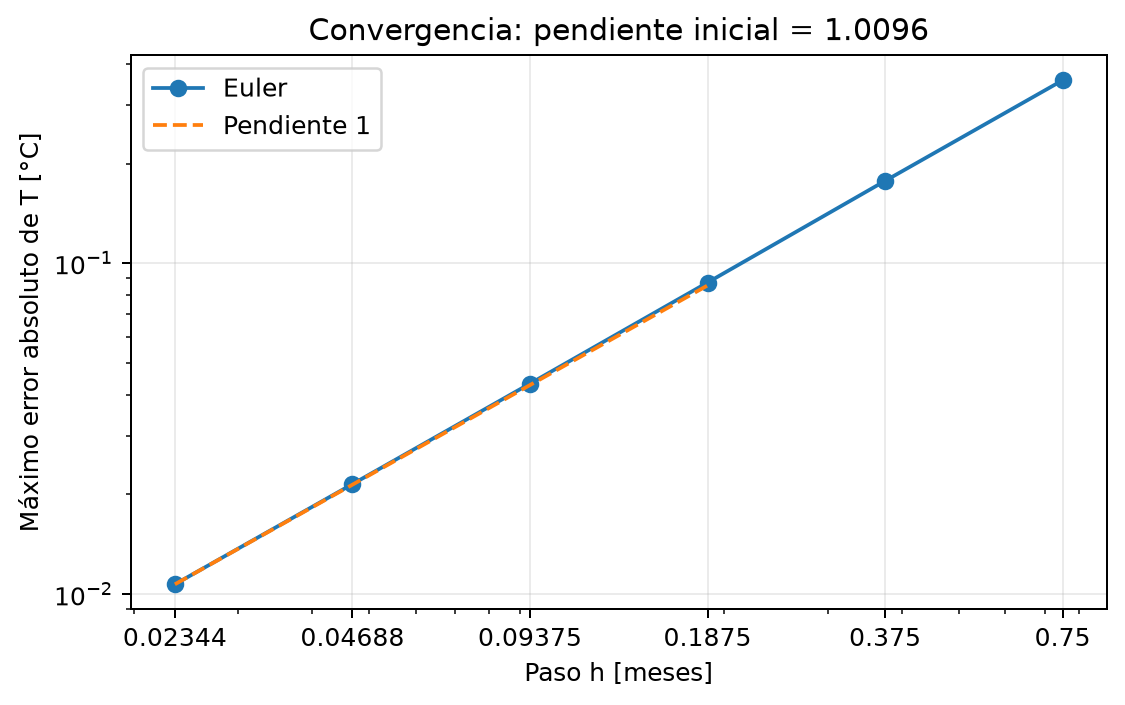
\includegraphics[width=0.85\textwidth]{img/01_convergencia.png}
    \caption{Error máximo absoluto de $T$ en función del paso temporal,
    en escala logarítmica en ambos ejes. La línea discontinua representa
    una dependencia de primer orden.}
    \label{figure:parte1-convergencia}
\end{figure}




\subsection{Estabilidad al aumentar el paso}
Se realizó un barrido auxiliar entre $0{,}25$ y $2$ meses, con un
incremento de $0{,}025$ meses. En este barrido se interpoló linealmente
la referencia en los tiempos de cada simulación cuando las mallas no
coincidían. Se examinó el cociente $E(h)/h$, aproximadamente constante
para errores de primer orden, y se compararon las curvas de precipitación
con la de referencia.


\begin{figure}[htbp]
    \centering
    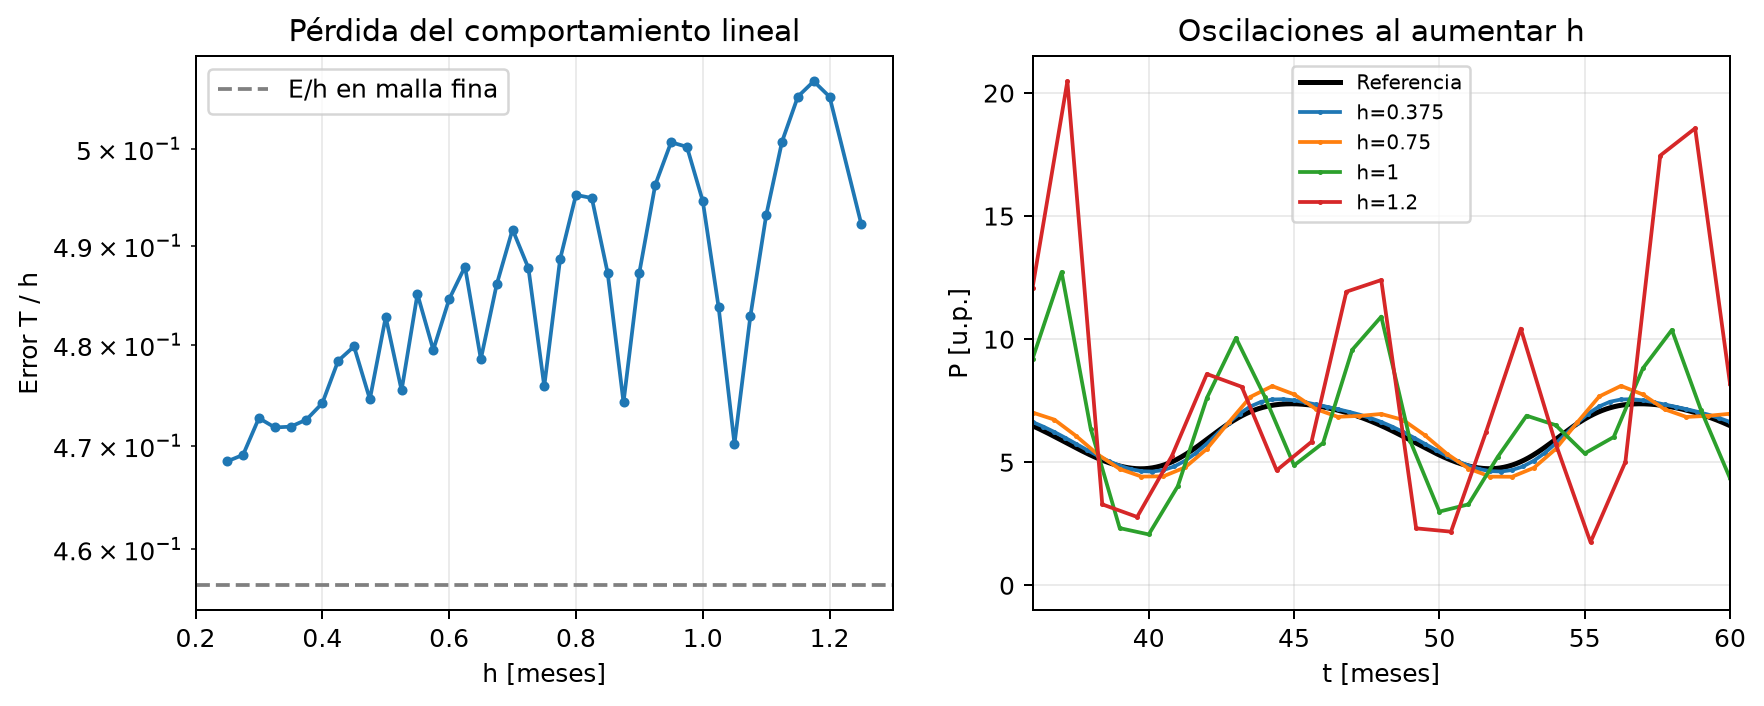
\includegraphics[width=\linewidth]{img/02_estabilidad.png}
    \caption{Cociente $E(h)/h$ para las trayectorias finitas del barrido
    auxiliar (izquierda) y comparación de $P(t)$ entre los meses 36 y 60
    para distintos pasos temporales (derecha).}
    \label{fig:parte1-estabilidad}
\end{figure}

El muestreo anterior no explicaba el crecimiento abrupto del error. Por eso se exploró el intervalo $[1{,}15;\,1{,}30]$ meses con un paso de $0{,}0001$ meses. Entre $h=1{,}1859$ y $h=1{,}1860$ meses, el error máximo de $T$ pasó de aproximadamente $0{,}696$ a
$4{,}42\times 10^{49}\;{}^\circ\mathrm{C}$. En ese segundo caso, la trayectoria ya era explosiva, aunque sus valores todavía se podían representar. El primer desbordamiento apareció en $h=1{,}1865$ meses. 
La Figura~\ref{fig:parte1-detalle} muestra que, en esta zona de
transición, pasos muy cercanos pueden dar comportamientos distintos.
Estos valores dependen de la resolución del barrido y del horizonte de
integración.

\begin{figure}[htbp]
    \centering
    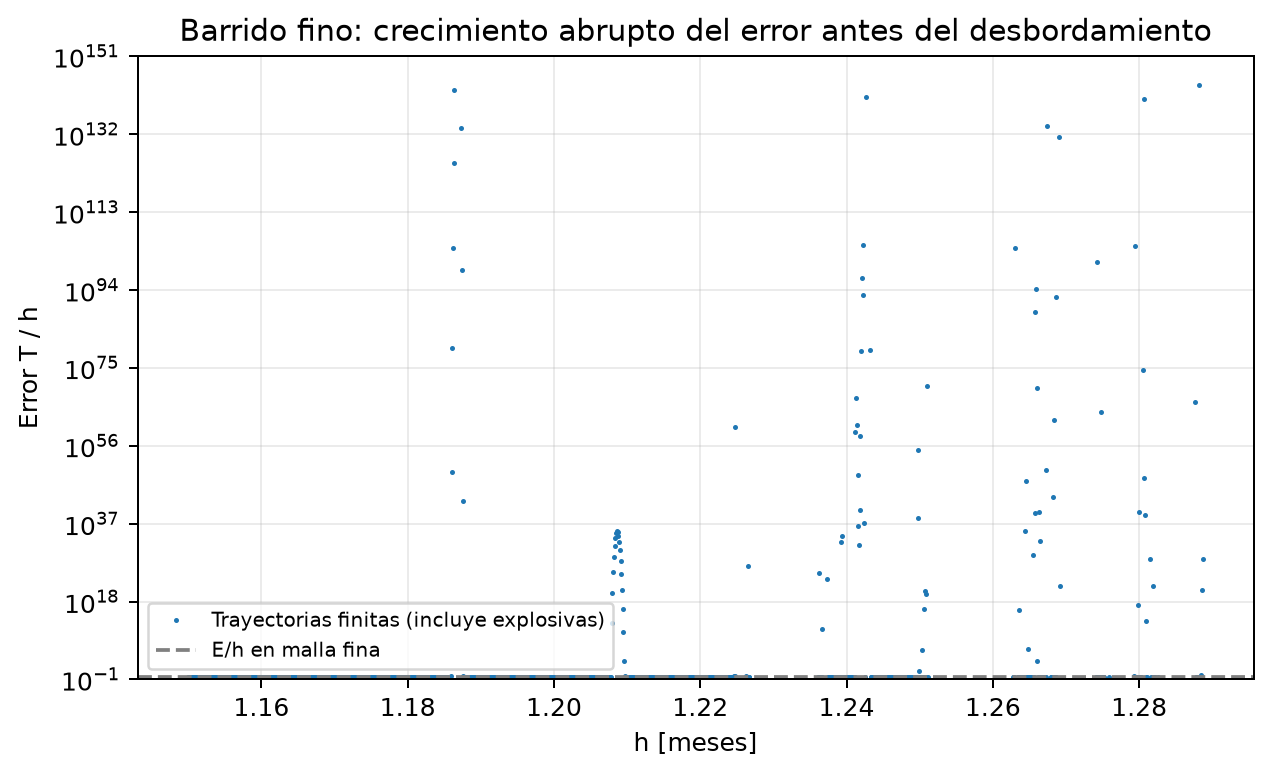
\includegraphics[width=0.90\linewidth]{img/08_estabilidad_detalle.png}
    \caption{Cociente $E(h)/h$ en el barrido fino. Se grafican las trayectorias que llegaron a 60 meses con valores finitos, incluidas las explosivas. Las simulaciones con desbordamiento no aparecen.}
    \label{fig:parte1-detalle}
\end{figure}

Para entender las oscilaciones, se linealizó el sistema alrededor de la trayectoria nominal. En un instante fijo, si $J$ es el jacobiano, una perturbación se propaga aproximadamente con la matriz $I+hJ$. Para un autovalor $\lambda$ de $J$ con parte real negativa, la condición
$|1+h\lambda|\leq 1$ da el límite local
\begin{equation}
    h\leq -\frac{2\operatorname{Re}(\lambda)}{|\lambda|^2}.
\end{equation}

El menor de estos límites, calculado en el último año de la trayectoria nominal, fue de aproximadamente $0{,}8422$ meses, y el autovalor que lo determina es complejo. Esto es coherente con lo observado: con $h=1$ y $h=1{,}2$ meses la precipitación ya oscila de forma artificial (Figura~\ref{fig:parte1-estabilidad}), y el salto abrupto del error aparece poco por encima de ese límite, cerca de $h=1{,}186$ meses. El límite es algo menor que el paso donde se observa el salto porque el cálculo es local: el jacobiano varía a lo largo de la trayectoria y se lo evaluó
``congelado'' en cada instante, de modo que no determina por sí solo la
estabilidad del sistema no lineal.

El error de discretización disminuye al refinar $h$. La inestabilidad
numérica, en cambio, aparece cuando $h$ supera el límite de estabilidad y se
manifiesta como oscilaciones artificiales y crecimiento explosivo, en lugar
de un error que crece de forma gradual con $h$. Una solución finita no es
necesariamente estable ni precisa: con $h=6$ y $h=12$ meses los resultados
fueron finitos, pero incompatibles con la referencia.





\newpage

\section{Parte 2: Severidad estacional, desfase y sensibilidad paramétrica}


\subsection{Selección del paso temporal y análisis general}

Para empezar esta segunda parte, seleccionamos un paso temporal lo suficientemente pequeño para que, de acuerdo con los resultados de la \textbf{Parte 1}, la solución producida sea precisa y estable. A partir de estos mismos resultados, elegimos:

\begin{equation}
    \boxed{h = 0{,}0029296875 \;\mathrm{meses}}.
\end{equation}

En todas las combinaciones exploradas y los barridos individuales, la última comparación h frente a 2h da una diferencia relativa máxima de SP de 0{,}1305\,\% y una diferencia máxima de desfase de 0{,}00878906 meses. Por lo tanto, consideramos el paso seleccionado lo suficientemente bueno para su utilización en los análisis posteriores.

Esta elección es coherente con la Parte~1: $h=12/4096$ es unas $290$ veces menor que el límite local de estabilidad ($0{,}84$ meses), pertenece al rango convergente, donde $E\approx0{,}457\,h$ predice un error máximo de $T$ de unos $1{,}3\times10^{-3}\;{}^\circ\mathrm{C}$, y la diferencia medida entre la simulación nominal con este paso y la referencia fue de $1{,}316\times10^{-3}\;{}^\circ\mathrm{C}$.

Los indicadores se calculan unicamente en el último ciclo anual, definido por el intervalo $48 \le t \le 60$ meses, y se define severidad estacional de las precipitaciones como:

\begin{equation}
    SP = \frac{P_{max} - P_{min}}{P_{med}}
\end{equation}


donde $P_{max}$, $P_{min}$ y $P_{med}$ son los valores máximo, mínimo y promedio de la precipitación durante el ultimo ciclo anual.

Por otra parte, el desfase temperatura-precipitación se calcula como:

\begin{equation}
    \triangle t_{TP} = t_{P,max} - t_{T,max}
\end{equation}

donde $t_{P,max}$ y $t_{T,max}$ corresponde al tiempo en el que se alcanzan la máxima precipitación y temperatura respectivamente.

\subsubsection{Comportamiento del modelo con los parámetros nominales}

En primer lugar, se decidió encontrar los SP y $\triangle t_{TP}$ y graficar T(t), H(t) y P(t) para los 60 meses de la simulación, con resultados:

Con los parámetros nominales, la simulación produce un ciclo anual
prácticamente repetitivo hacia el final del intervalo de integración. El
residuo anual máximo fue $4{,}05\times10^{-4}$, valor inferior al umbral
adoptado de $0{,}01$.

\begin{table}[H]
    \centering
    \small
    \caption{Indicadores del escenario nominal durante el último ciclo anual.}
    \label{tab:parte2-nominal}
    \begin{tabular}{@{} c c c c c c @{}}
        \toprule
        $SP$ & $\Delta t_{TP}$ [meses] & $P_{\max}$ [u.p.] &
        $P_{\min}$ [u.p.] & $P_{\mathrm{med}}$ [u.p.] &
        Residuo anual \\
        \midrule
        $0{,}428658$ & $0{,}826172$ & $7{,}37594$ &
        $4{,}73548$ & $6{,}15985$ & $4{,}05214\times10^{-4}$ \\
        \bottomrule
    \end{tabular}
\end{table}

El máximo de precipitación ocurre aproximadamente $0{,}83$ meses después
del máximo de temperatura. Esto es consistente con la estructura del
modelo, ya que el aumento de temperatura incrementa la humedad mediante
el término $\beta T^2$, y posteriormente la humedad alimenta la variable
de precipitación mediante el término $\delta H^2$.

\begin{figure}[H]
    \centering
    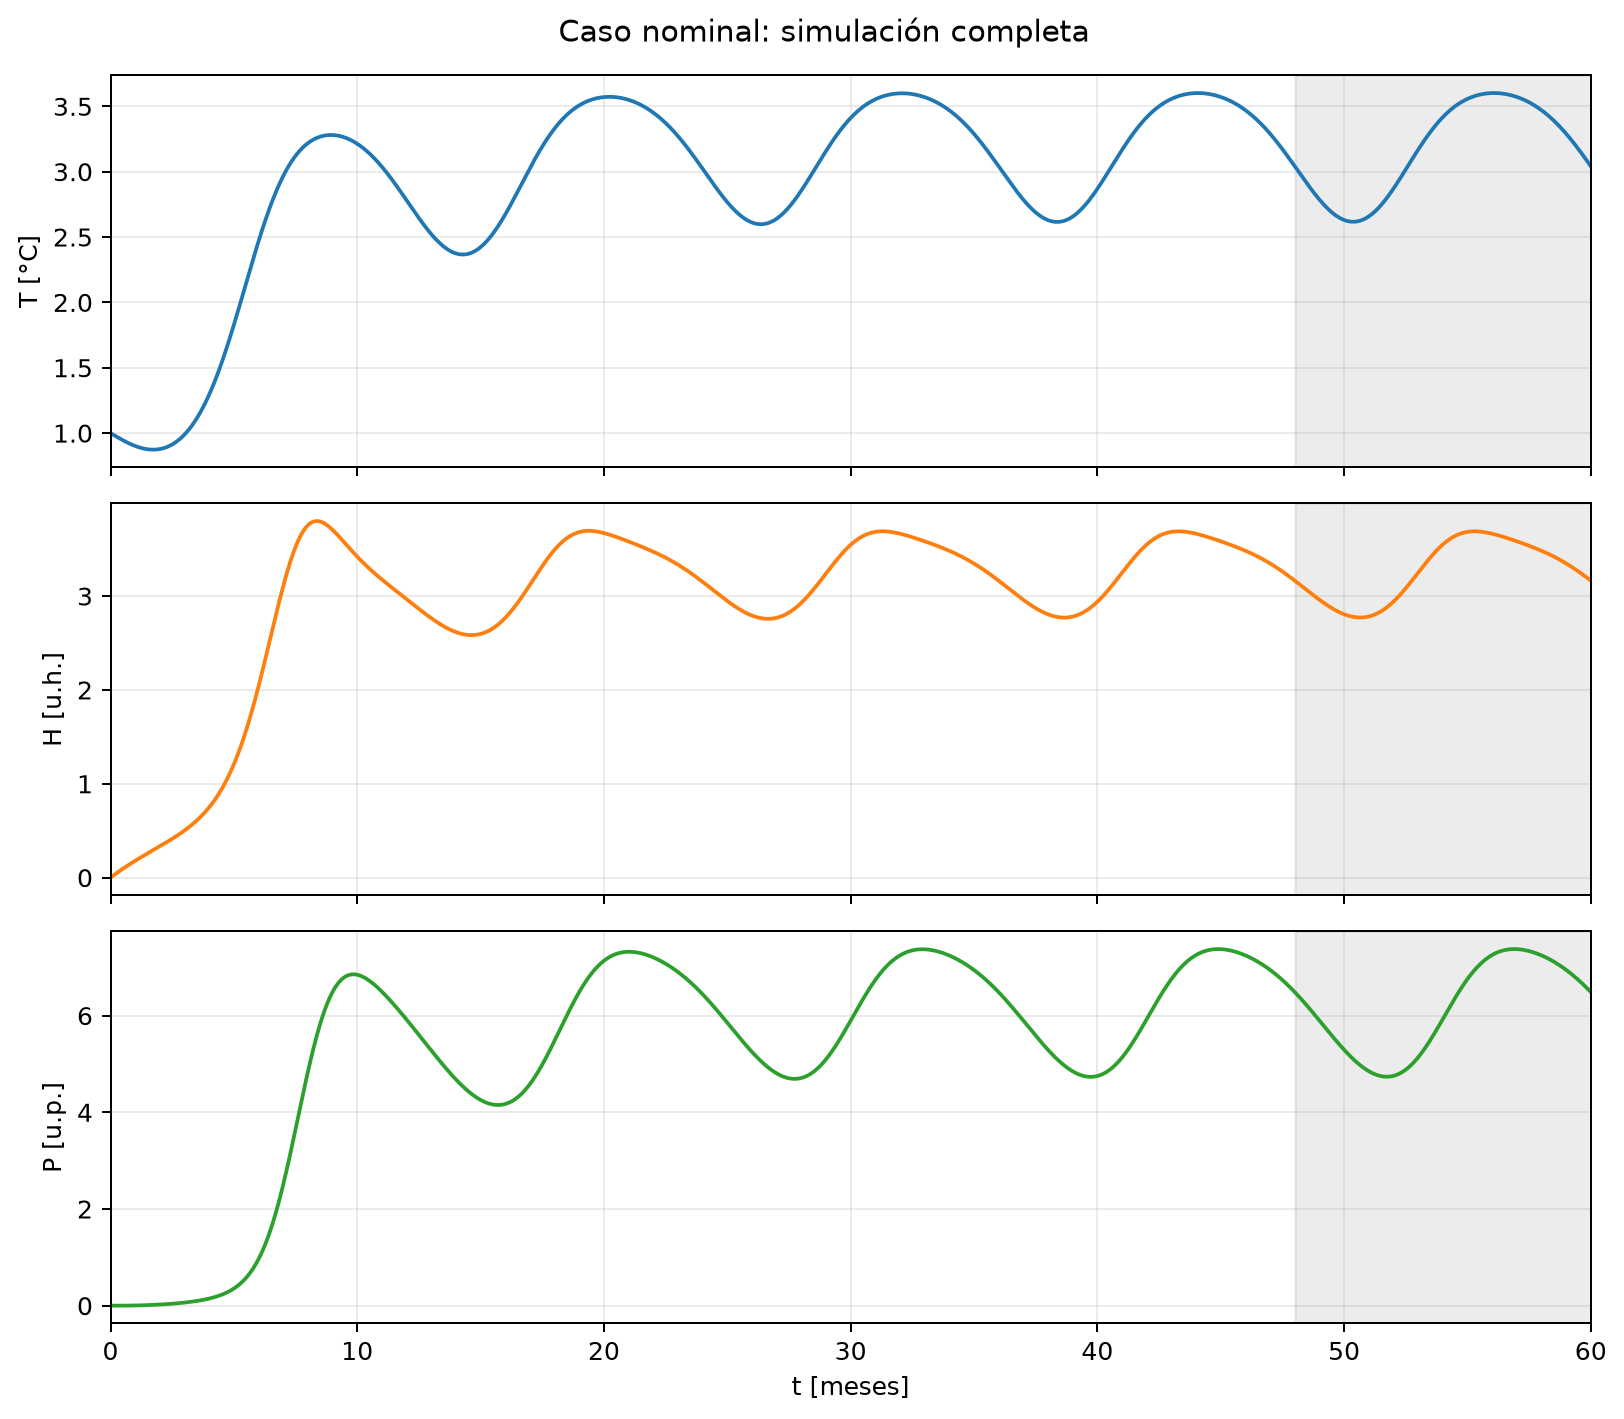
\includegraphics[width=\linewidth]{img/03_nominal_60_meses.png}
    \caption{Evolución temporal de $T(t)$, $H(t)$ y $P(t)$ durante los
    $60$ meses de simulación para los parámetros nominales.}
    \label{fig:parte2-nominal-completo}
\end{figure}


\begin{figure}[H]
    \centering
    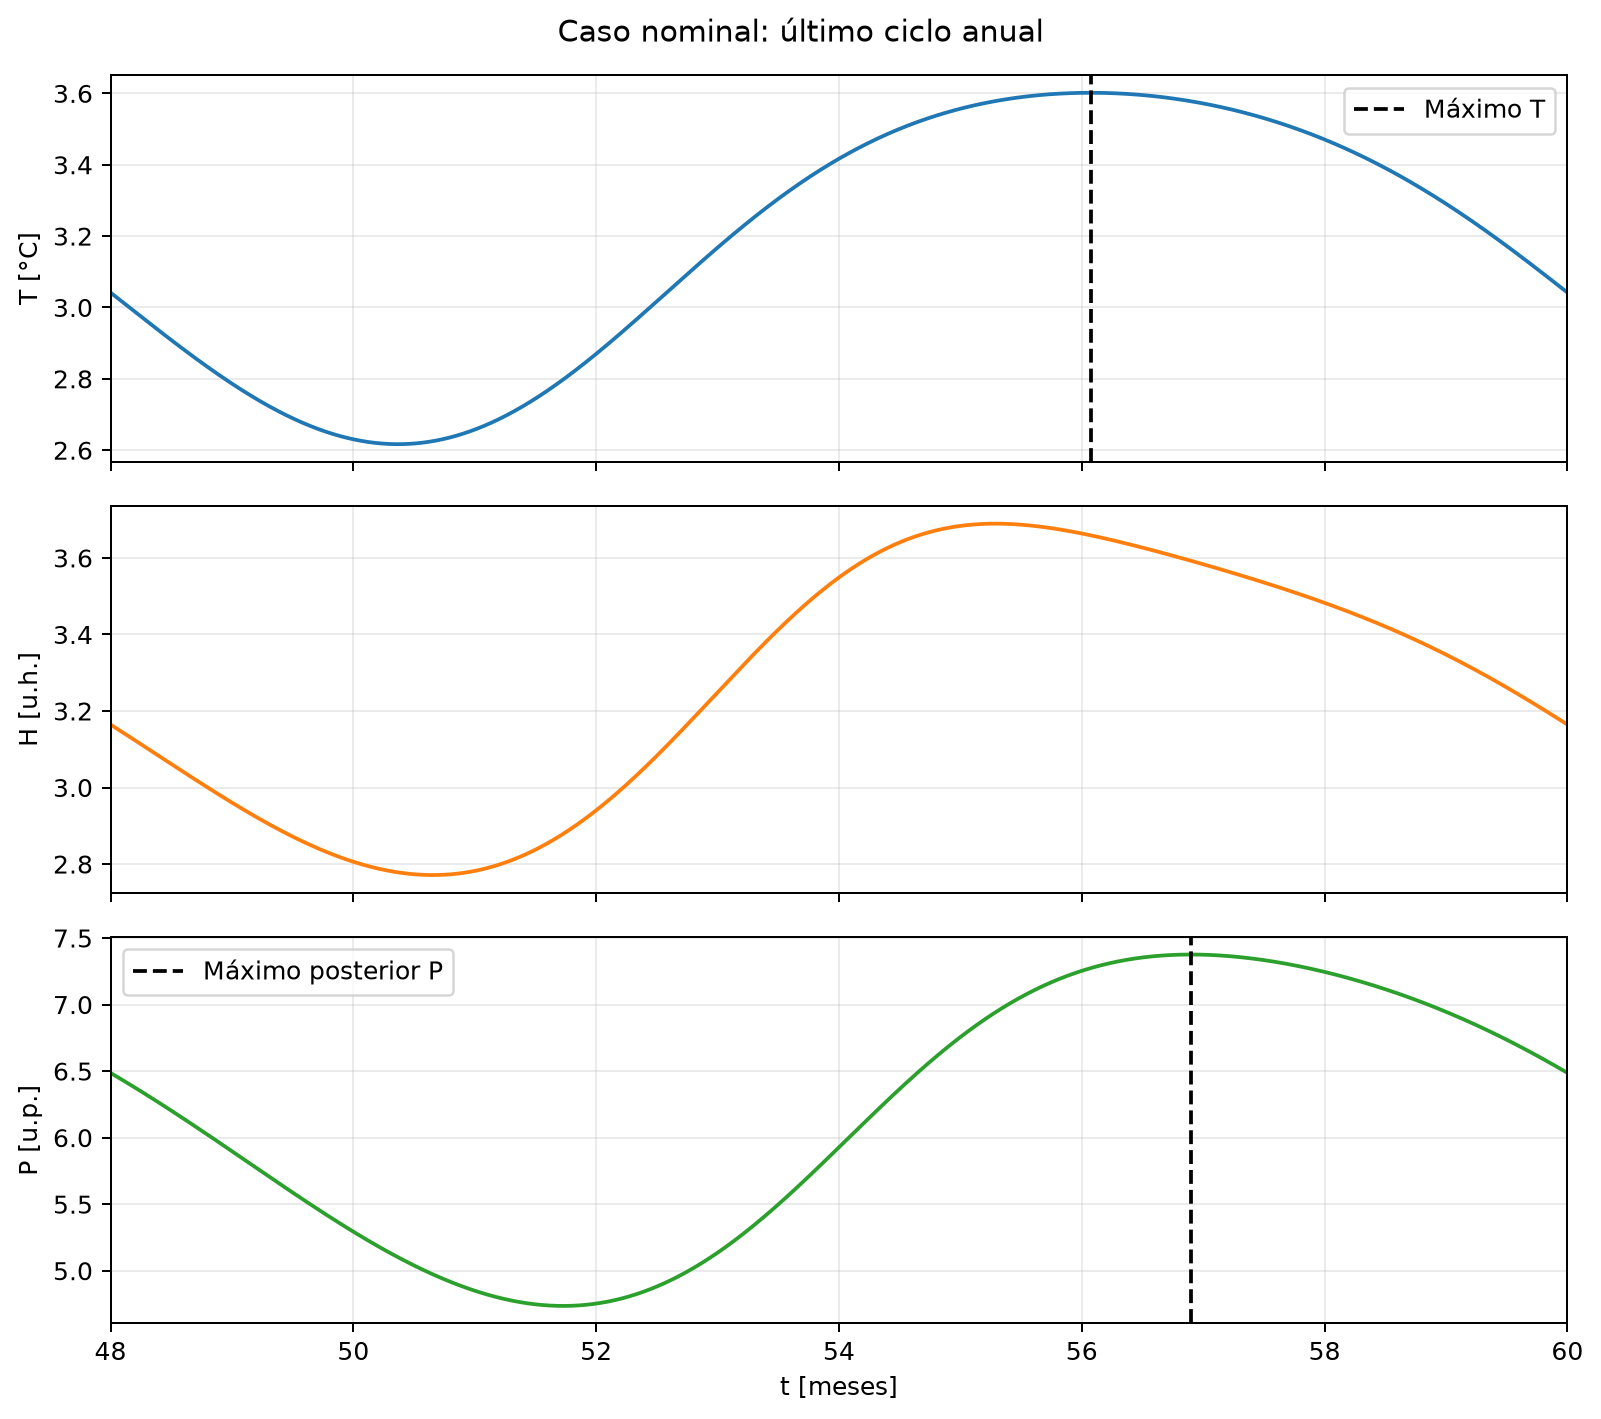
\includegraphics[width=\linewidth]{img/04_nominal_ultimo_ciclo.png}
    \caption{Último ciclo anual del escenario nominal. Se observa el
    desfase entre los máximos de temperatura y precipitación.}
    \label{fig:parte2-nominal-ciclo}
\end{figure}


\subsubsection{Sensibilidad paramétrica individual}

Se estudió la influencia de los parámetros $A$, $\beta$, $\gamma$ y
$\sigma$ sobre la severidad estacional. En cada barrido se modificó un
único parámetro, manteniendo los restantes en sus valores nominales.

\begin{table}[H]
    \centering
    \small
    \caption{Variación de la severidad estacional y del desfase en los
    barridos individuales.}
    \label{tab:parte2-sensibilidad}
    \begin{tabular}{@{} c c c c c @{}}
        \toprule
        Parámetro & Intervalo explorado & $SP$ mínimo & $SP$ máximo &
        Desfase mínimo--máximo [meses] \\
        \midrule
        $A$ & $0{,}25$--$0{,}60$ & $0{,}215492$ & $0{,}626963$ &
        $0{,}735352$--$0{,}955078$ \\
        $\beta$ & $0{,}10$--$0{,}30$ & $0{,}339406$ & $0{,}485561$ &
        $0{,}685547$--$1{,}312500$ \\
        $\gamma$ & $0{,}05$--$0{,}20$ & $0{,}334136$ & $0{,}548950$ &
        $0{,}670898$--$1{,}174805$ \\
        $\sigma$ & $0{,}40$--$1{,}00$ & $0{,}341011$ & $0{,}480803$ &
        $0{,}773438$--$1{,}195312$ \\
        \bottomrule
    \end{tabular}
\end{table}

En los puntos muestreados, SP aumenta con A, $\beta$ y $\sigma$, y disminuye con $\gamma$. El desfase no aumenta al incrementar ninguno de los cuatro parámetros; algunos valores consecutivos coinciden por la resolución temporal de los picos. Estas tendencias se refieren a los intervalos indicados y al resto de parámetros nominales.

\begin{itemize}
        \item A: aumenta el contraste estacional de R(t), sin cambiar su media anual. En los experimentos aumenta SP y disminuye el desfase: la excitación térmica más intensa se propaga a H y P a través de sus fuentes cuadráticas.
        \item $\beta$: aumenta la fuente de humedad $\beta T^2$. En este rango aumenta SP y reduce el desfase, aunque también refuerza el enfriamiento indirecto de T a través de H. El resultado surge del sistema acoplado, no solo del signo positivo de beta.
        \item $\gamma$: aumenta el consumo de humedad $\gamma H P$. Reduce la humedad disponible para la fuente $\delta H^2$. Se observa una menor severidad relativa y un desfase menor; el consumo atenúa el ciclo y acelera el ajuste de humedad cuando P es positiva.
        \item $\sigma$: aumenta la descarga de P y reduce su escala de disipación 1/sigma. En este rango disminuye el desfase y aumenta SP: una disipación más rápida reduce el almacenamiento y permite mayor contraste relativo entre máximo y mínimo. Esto no implica que aumente la precipitación absoluta.
\end{itemize}

\begin{figure}[H]
    \centering
    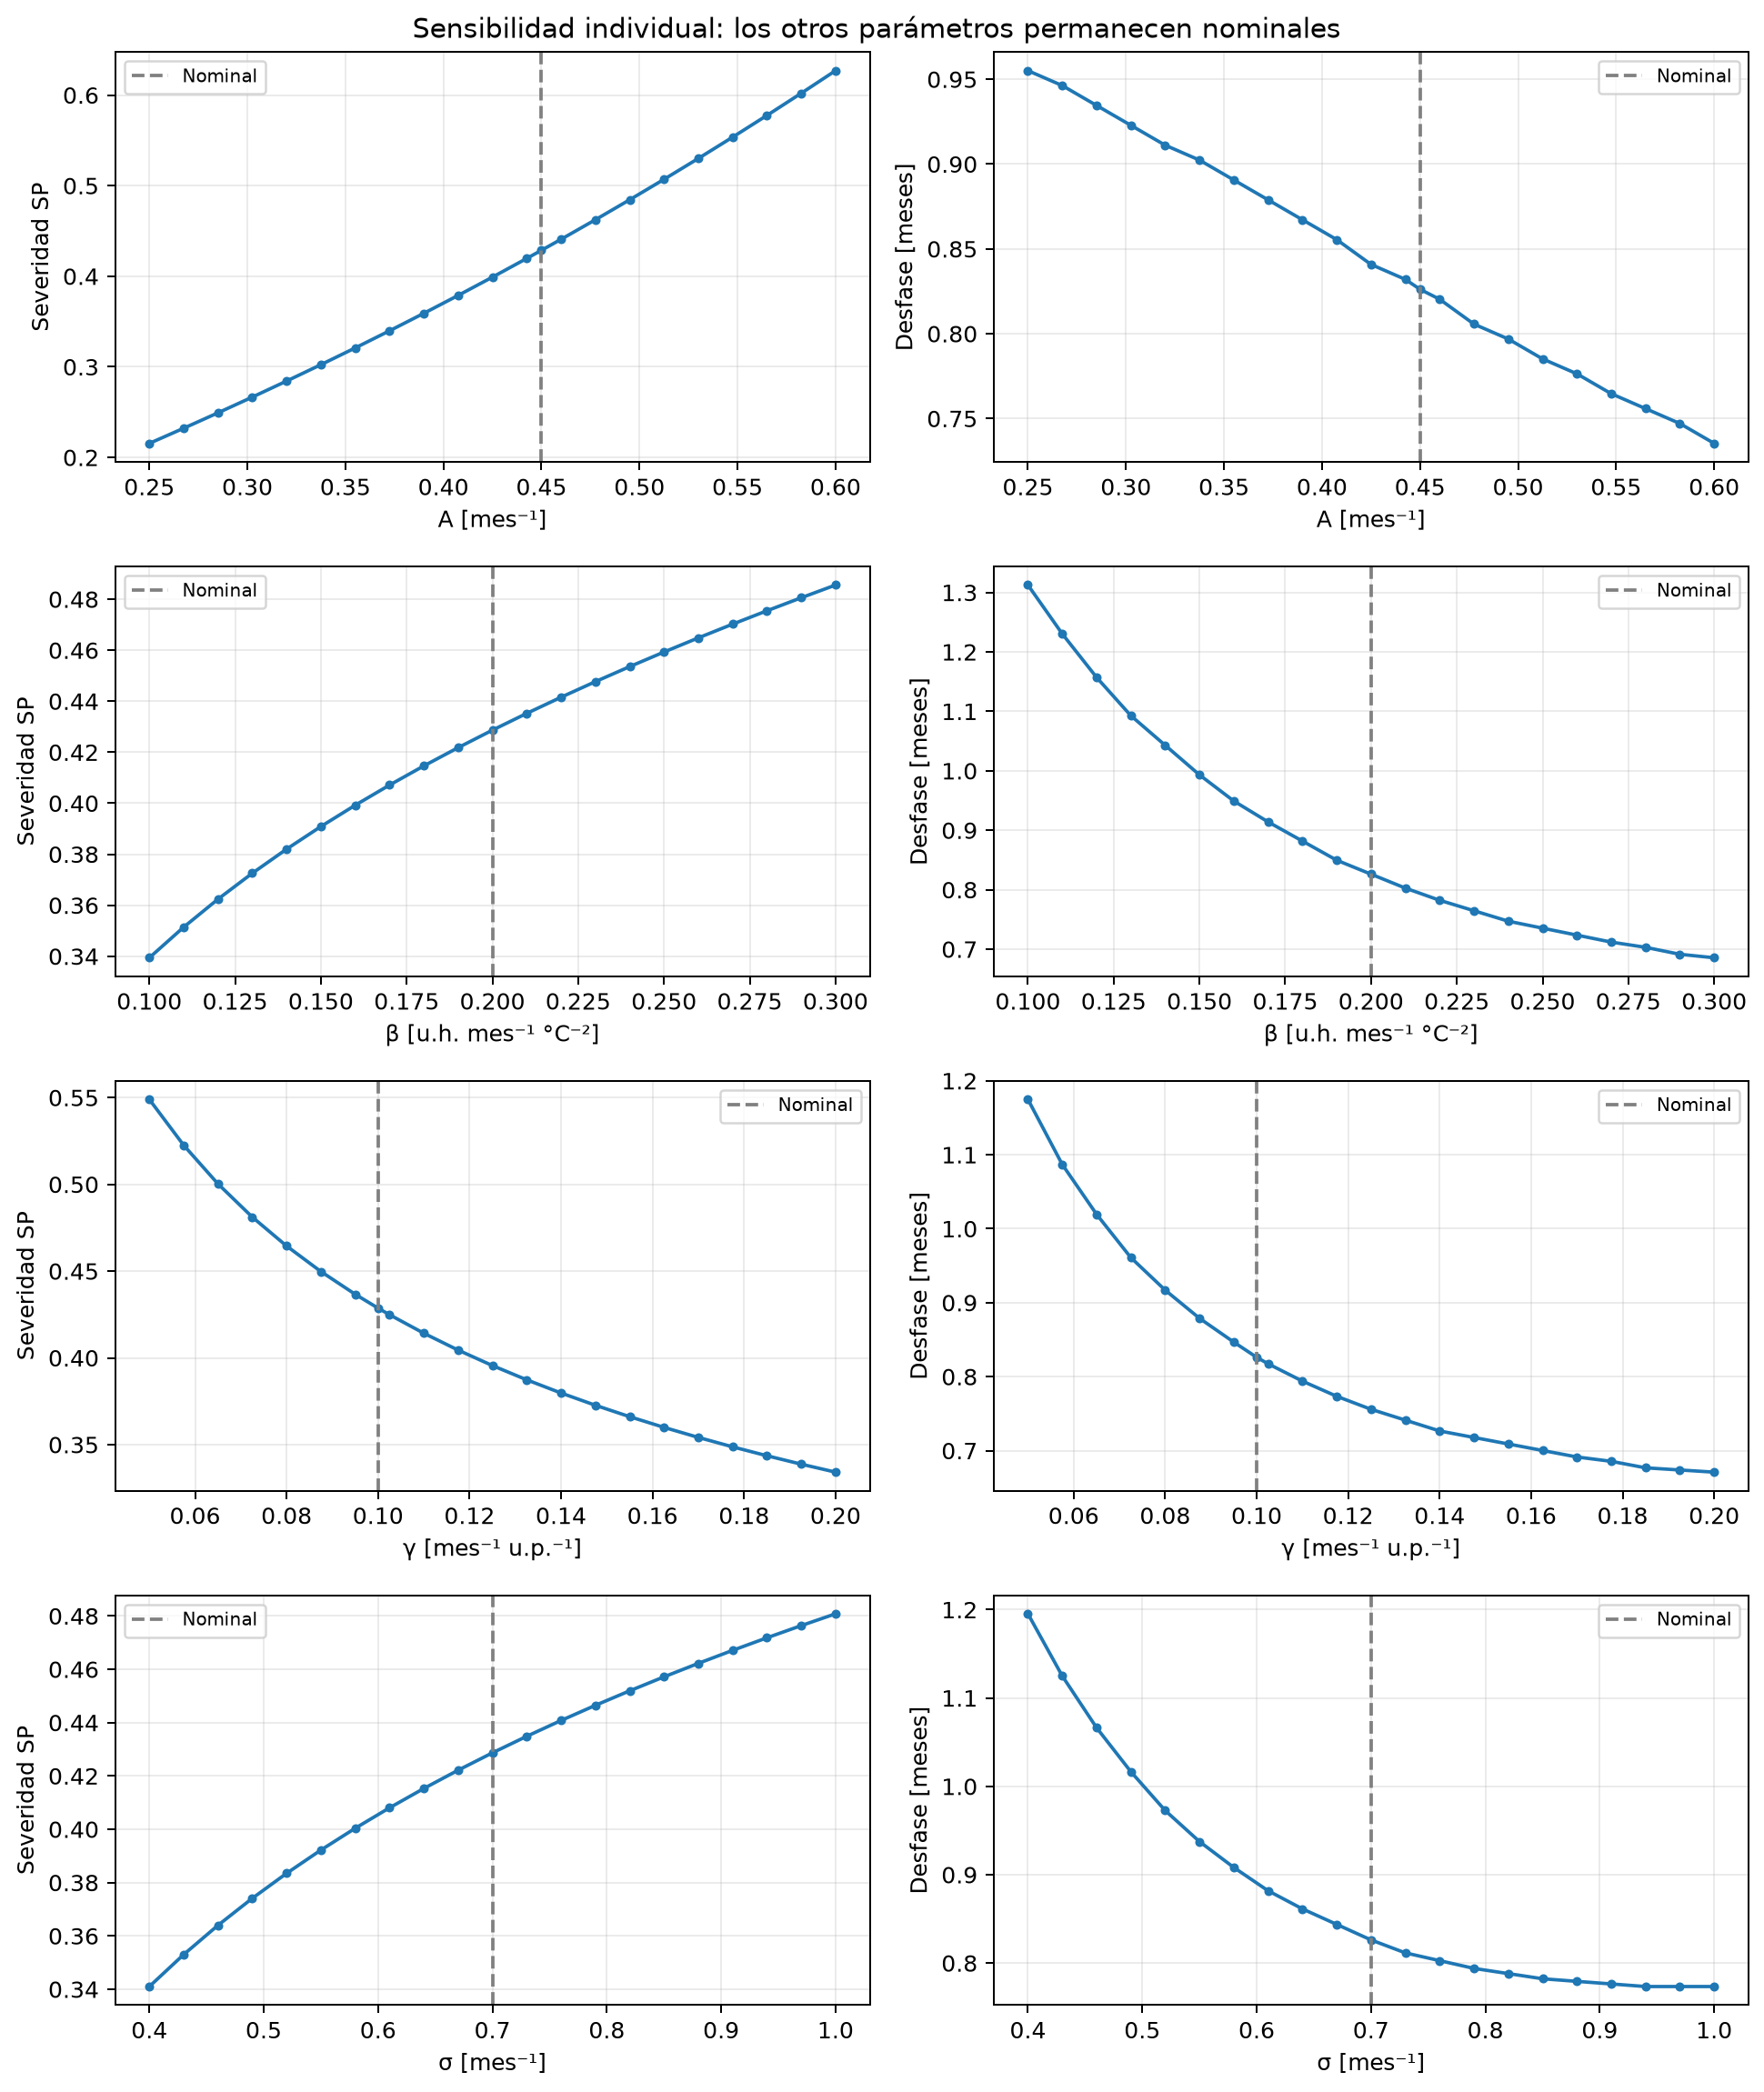
\includegraphics[width=\linewidth]{img/05_sensibilidad.png}
    \caption{Sensibilidad de la severidad estacional y del desfase ante
    variaciones individuales de $A$, $\beta$, $\gamma$ y $\sigma$.}
    \label{fig:parte2-sensibilidad}
\end{figure}


\subsubsection{Búsqueda conjunta y comparación con el escenario nominal}

Luego de los barridos individuales, se modificaron simultáneamente los parámetros $A$, $\beta$, $\gamma$ y $\sigma$ con el objetivo de maximizar la severidad estacional, manteniendo una solución acotada y aproximadamente periódica durante el último ciclo anual.

Se evaluaron 7170 combinaciones distintas entre la grilla inicial de $5^4=625$ puntos, una grilla global de $9^4=6561$ puntos y el refinamiento local de $5^4=625$ puntos eliminando los repetidos. Todas cumplieron el criterio operativo de admisibilidad. El mayor residuo
anual registrado fue $0{,}00110776$ menor que el umbral adoptado de
$0{,}01$.

El residuo compara cada variable del penúltimo y último ciclo a igual fase y normaliza por su máxima magnitud en el último ciclo. La comparación indica repetición anual aproximada al final de los 60 meses; no demuestra periodicidad exacta ni acotación para todo tiempo futuro.

La mejor combinación encontrada fue
\[
    \boxed{
    A=0{,}60,\qquad
    \beta=0{,}30,\qquad
    \gamma=0{,}05,\qquad
    \sigma=1{,}00.}
\]

\begin{table}[H]
    \centering
    \small
    \caption{Comparación de indicadores para distintos escenarios.}
    \label{tab:parte2-comparacion}
    \begin{tabular}{@{} l c c c c c c c c c @{}}
        \toprule
        Escenario & $A$ & $\beta$ & $\gamma$ & $\sigma$ &
        $SP$ & $\Delta t_{TP}$ [meses] & $P_{\max}$ [u.p.] &
        $P_{\min}$ [u.p.] & $P_{\mathrm{med}}$ [u.p.] \\
        \midrule
        Nominal
        & $0{,}45$ & $0{,}20$ & $0{,}10$ & $0{,}70$
        & $0{,}428658$ & $0{,}826172$ & $7{,}376$ & $4{,}736$ & $6{,}160$ \\
        Máxima severidad
        & $0{,}60$ & $0{,}30$ & $0{,}05$ & $1{,}00$
        & $0{,}991270$ & $0{,}893555$ & $12{,}653$ & $4{,}329$ & $8{,}397$ \\
        Todos máximos
        & $0{,}60$ & $0{,}30$ & $0{,}20$ & $1{,}00$
        & $0{,}626015$ & $0{,}439453$ & $5{,}450$ & $2{,}773$ & $4{,}275$ \\
        \bottomrule
    \end{tabular}
\end{table}

El escenario de máxima severidad tiene un valor de $SP$ aproximadamente
$2{,}31$ veces mayor que el escenario nominal. Sin embargo, este resultado
no se obtiene asignando el valor máximo a todos los parámetros.

La mejor combinación usa el valor mínimo de $\gamma$, ya que este parámetro
representa el consumo de humedad por precipitación. Al disminuir $\gamma$,
queda más humedad disponible para generar precipitación y aumenta la
severidad estacional.

De hecho, cuando todos los parámetros toman sus valores máximos se obtiene
$SP=0{,}626015$, un valor menor que el máximo encontrado. Esto muestra que
los parámetros actúan de forma acoplada y que aumentar cada uno por separado
no necesariamente aumenta la severidad estacional.

\begin{figure}[H]
    \centering
    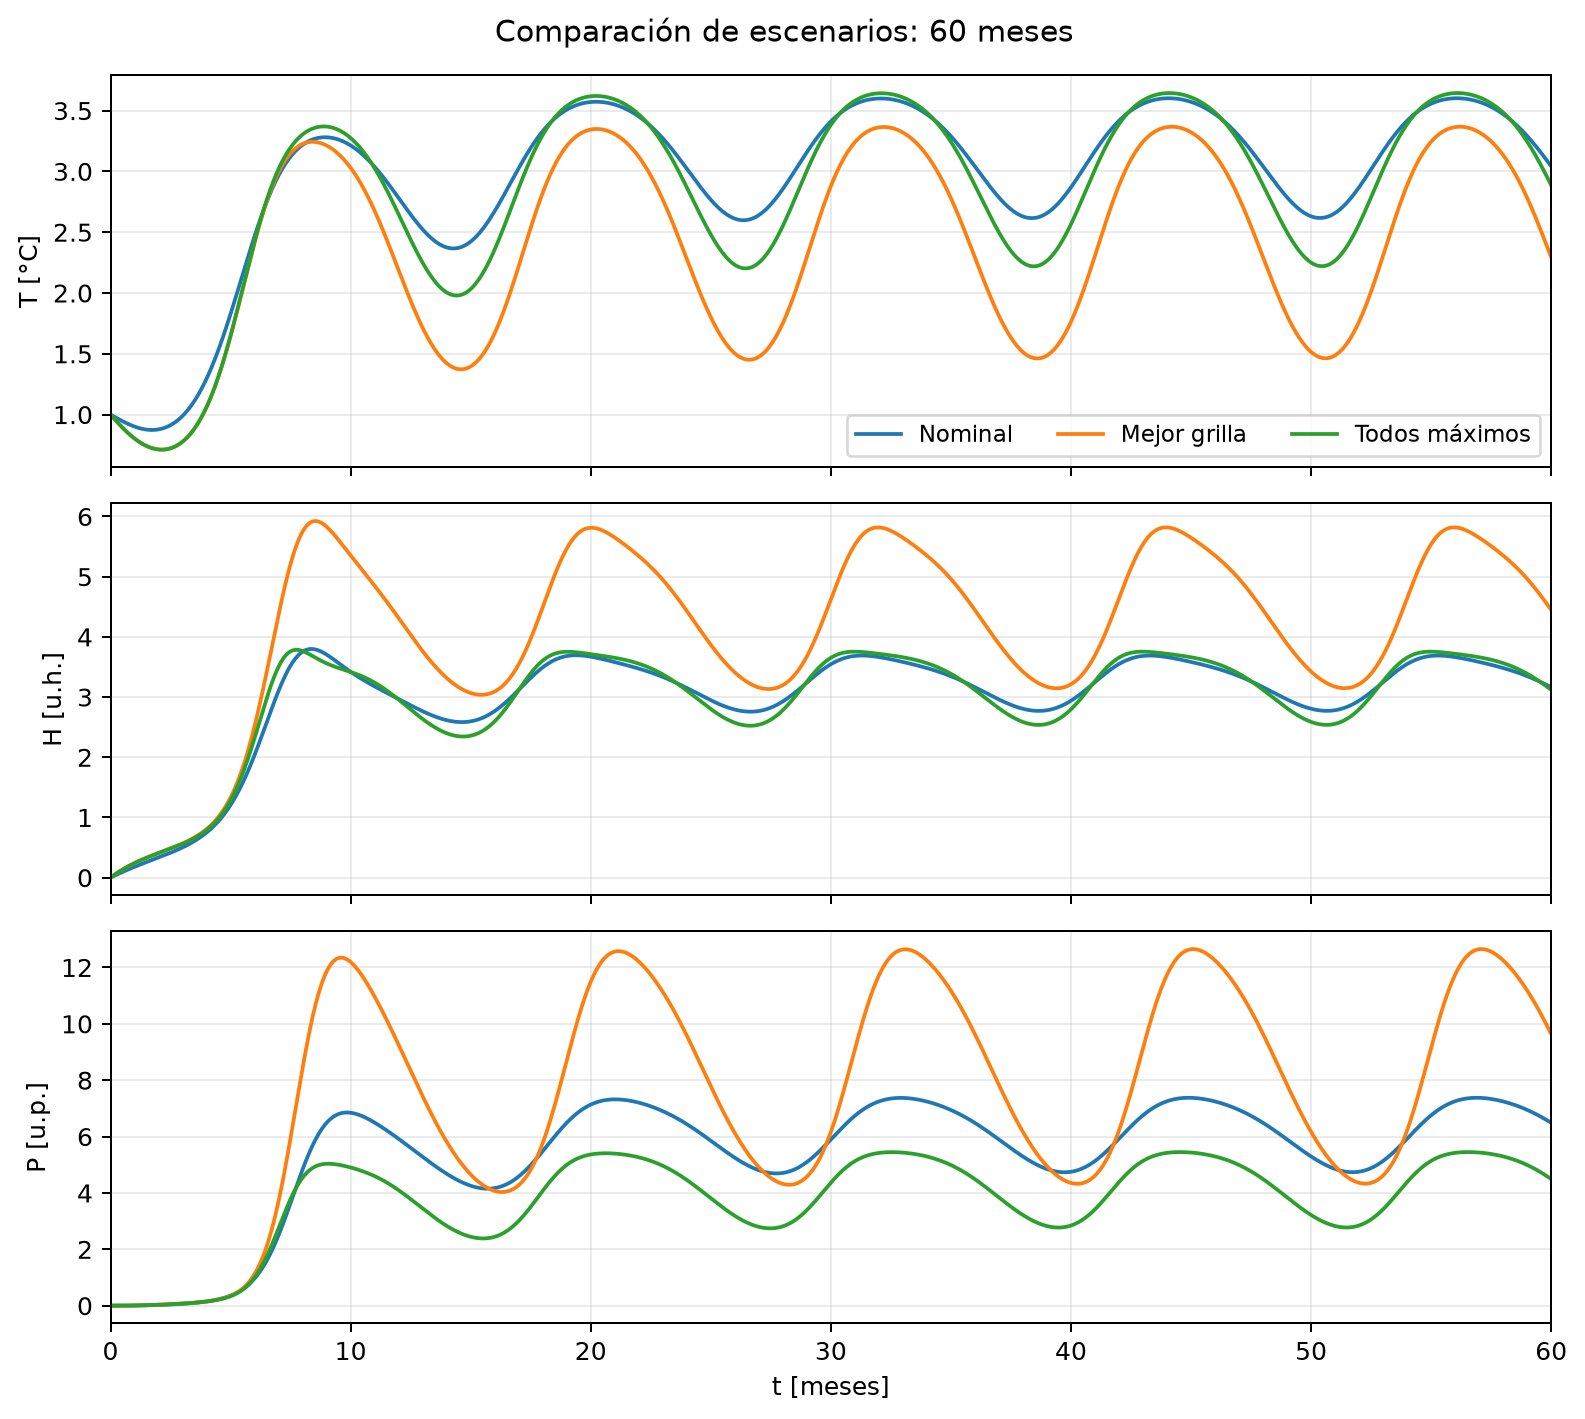
\includegraphics[width=\linewidth]{img/06_comparacion_60_meses.png}
    \caption{Comparación temporal entre el escenario nominal y el
    escenario de máxima severidad durante los $60$ meses simulados.}
    \label{fig:parte2-comparacion-completa}
\end{figure}

\begin{figure}[H]
    \centering
    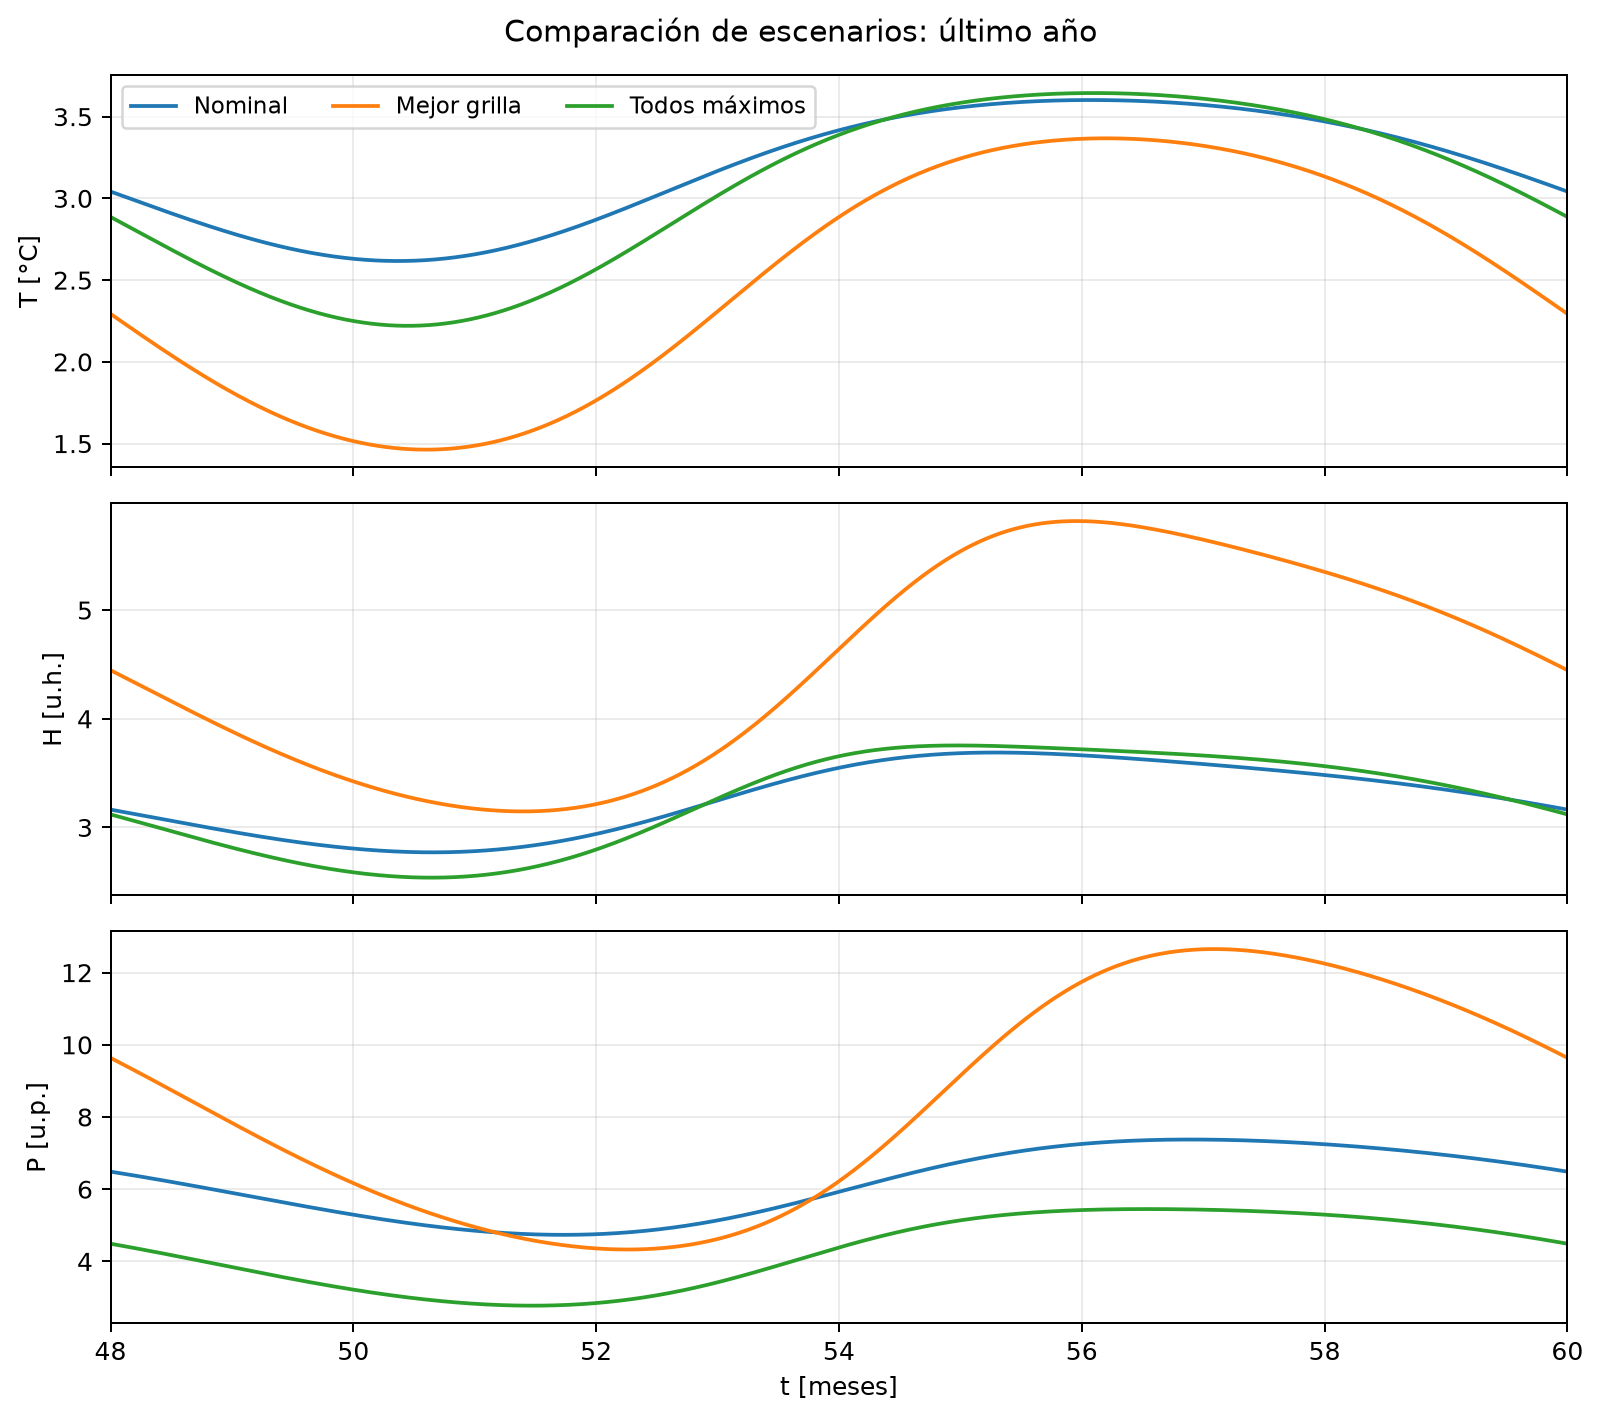
\includegraphics[width=\linewidth]{img/07_comparacion_ultimo_ciclo.png}
    \caption{Comparación entre el escenario nominal y el escenario de
    máxima severidad durante el último ciclo anual.}
    \label{fig:parte2-comparacion-ciclo}
\end{figure}

\begin{figure}[H]
    \centering
    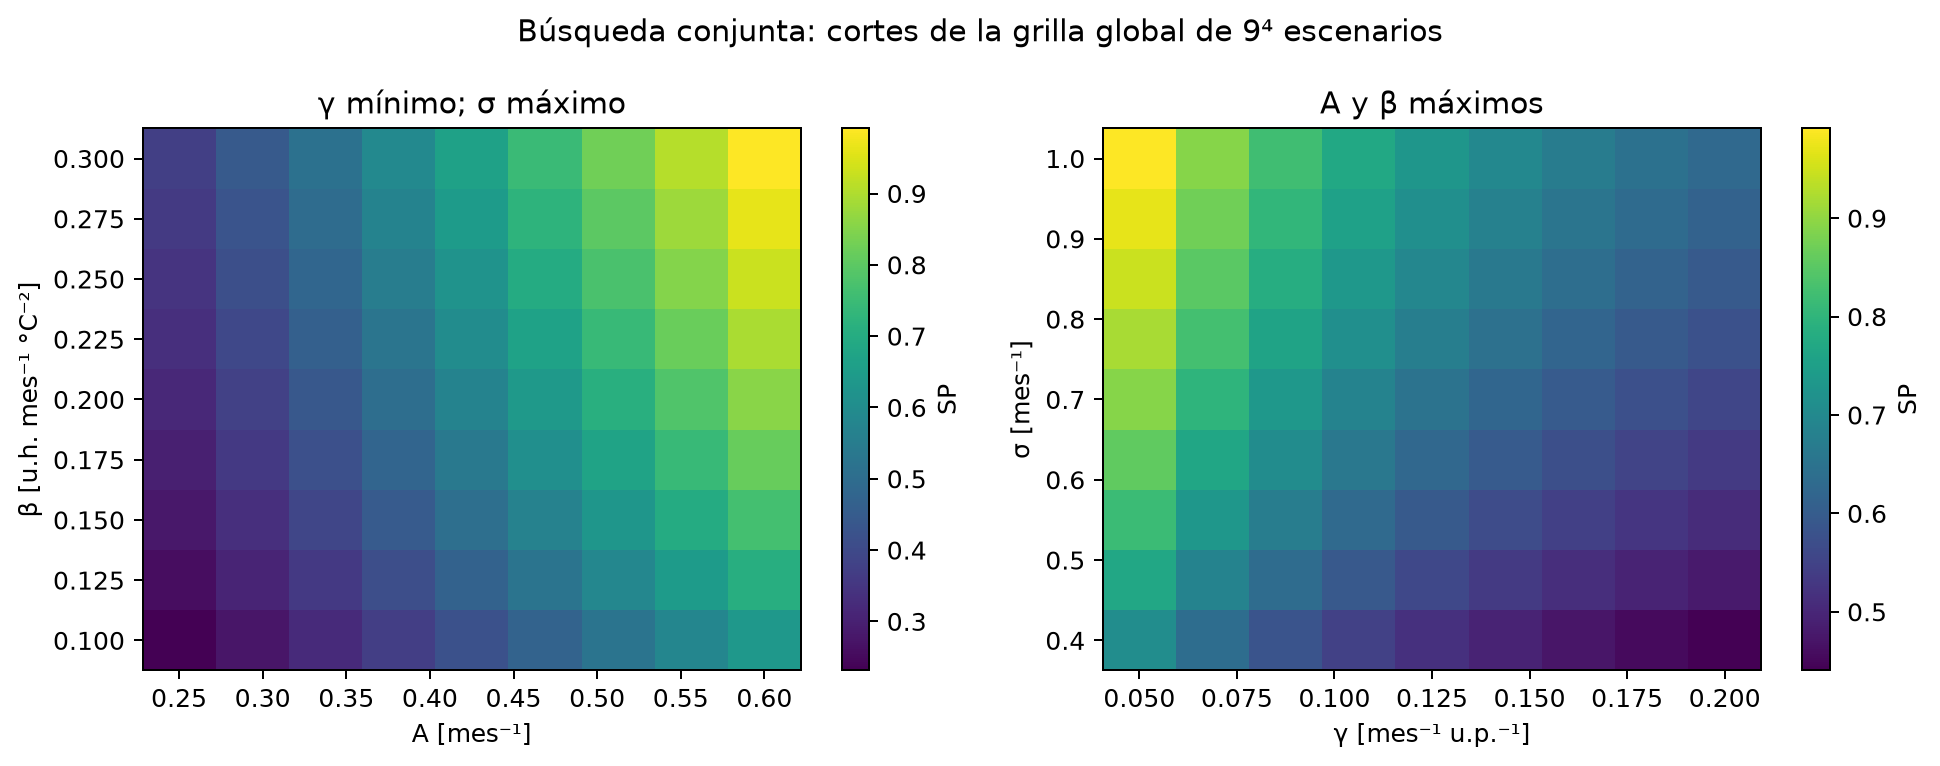
\includegraphics[width=\linewidth]{img/09_busqueda_conjunta.png}
    \caption{Resultados de la búsqueda conjunta. Los cortes mostrados
    mantienen fijos los otros dos parámetros según se indica en cada gráfico.}
    \label{fig:parte2-busqueda-conjunta}
\end{figure}

El mejor escenario tiene $S_P=0{,}9913$, unas $2{,}31$ veces el nominal, con
$P_{\max}$ y $P_{\mathrm{med}}$ mayores y un desfase similar
($0{,}894$ frente a $0{,}826$ meses). Sin embargo, \textbf{no} corresponde a
tomar todos los parámetros en su valor máximo: con $\gamma=0{,}20$ se obtiene
$S_P=0{,}626$, solo $1{,}46$ veces el nominal. El signo y la función de cada
término explican por qué:
\begin{itemize}
    \item $A$ multiplica $\cos(\omega t-\pi)$ en $R(t)$, que impulsa a $T$.
    Aumentarlo intensifica la oscilación de $T$, que se transmite a $H$ y $P$
    por las fuentes cuadráticas. Efecto positivo sobre $S_P$.
    \item $\beta$ multiplica $+\beta T^2$ en $dH/dt$: es una fuente de
    humedad. Efecto positivo.
    \item $\sigma$ multiplica $-\sigma P$ en $dP/dt$: es un sumidero de $P$.
    Al aumentarlo, $P$ sigue más rápido a $\delta H^2$ y el contraste entre
    máximo y mínimo crece. Efecto positivo.
    \item $\gamma$ multiplica $-\gamma HP$ en $dH/dt$: es un sumidero de
    humedad que crece con $P$. Aumentarlo reduce $H$, y con ella la fuente
    $\delta H^2$ de $P$. Efecto negativo.
\end{itemize}
Por lo tanto, $S_P$ crece al aumentar $A$, $\beta$ y $\sigma$ y al disminuir
$\gamma$, de modo que el máximo se alcanza con $\gamma$ en su mínimo. Además,
$S_P$ mide una amplitud relativa y no la cantidad de lluvia: con todos los
parámetros en su máximo, $P_{\max}=5{,}450$ u.p.\ es menor que el nominal
($7{,}376$ u.p.), aunque $S_P$ sea mayor.

El mejor escenario es el mejor entre los valores evaluados: las tres grillas
(inicial, global y local) dieron el mismo ganador, pero, como solo se
probaron valores discretos de los parámetros, esto no demuestra que sea el
máximo absoluto de $S_P$ dentro de los intervalos.
\newpage
\section{Conclusiones}

\textbf{Parte 1:}
\begin{itemize}
    \item Con una referencia de Euler de paso $h_{\mathrm{ref}}=12/2^{18}$,
    el error máximo de $T$ disminuyó de forma proporcional a $h$ en el rango
    convergente. Los órdenes observados estuvieron entre $1{,}006$ y $1{,}021$
    y la pendiente del ajuste log-log fue $1{,}0096$, compatibles con el orden
    $1$ esperado para Euler explícito.
    \item Al aumentar el paso, el error dejó de ser proporcional a $h$ y
    apareció crecimiento explosivo. En el barrido fino, el error máximo de $T$
    pasó de $0{,}696$ a $4{,}42\times10^{49}\;{}^\circ\mathrm{C}$ entre
    $h=1{,}1859$ y $h=1{,}1860$ meses, y el primer desbordamiento apareció
    en $h=1{,}1865$ meses. Esta zona de transición es irregular: pasos muy
    cercanos dan comportamientos distintos, por lo que estos valores no son un
    umbral exacto.
    \item El error de discretización disminuye al refinar $h$. La inestabilidad
    numérica, en cambio, se manifiesta como oscilaciones artificiales y
    crecimiento explosivo que no se corrigen refinando poco el paso. Una
    solución finita no es necesariamente estable ni precisa: con $h=6$ y
    $h=12$ meses los resultados fueron finitos, pero incompatibles con la
    referencia.
\end{itemize}


\textbf{Parte 2
:}
\begin{itemize}
    \item Con $h=12/4096$ meses, muy por debajo de la zona de inestabilidad,
    los indicadores cambiaron como máximo $0{,}1305\,\%$ en $S_P$ y $0{,}0088$
    meses en el desfase al duplicar el paso. En el caso nominal, $S_P=0{,}4287$ y $\Delta t_{TP}=0{,}826$ meses.
    \item En los barridos individuales, $S_P$ aumenta con $A$, $\beta$ y
    $\sigma$ y disminuye con $\gamma$, y el desfase disminuye al aumentar
    cualquiera de los cuatro. $A$ es el que más modifica $S_P$.
    \item De las $7170$ combinaciones evaluadas, la que maximiza $S_P$ es
    $(A,\beta,\gamma,\sigma)=(0{,}60;\,0{,}30;\,0{,}05;\,1{,}00)$, con
    $S_P=0{,}9913$, unas $2{,}31$ veces el nominal.
    \item Ese escenario \textbf{no} es el de todos los parámetros en su
    máximo: $\gamma$ es un sumidero de humedad y debe estar en su mínimo.
    Con todos en su máximo, $S_P=0{,}6260$.
\end{itemize}

\textbf{Limitaciones.} El mejor escenario es el mejor entre los valores
evaluados, no un máximo absoluto demostrado. La repetición anual se verificó
con dos ciclos y una tolerancia, y el modelo es una simplificación sin ajuste
a datos observados, por lo que no constituye un pronóstico climático.
\newpage
\appendix
\section{Uso de IA}

Utilizamos la IA como asistencia para desarrollar el código en Python a partir de nuestra propuesta inicial. La herramienta colaboró con la implementación del método de Euler, la automatización de barridos de pasos y parámetros, el cálculo de indicadores y la generación de gráficos.

Prompt utilizado: 

\begin{quote}
"Según nuestra base de código y el PDF, ayudando a desarrollar un código claro, comentado y reutilizable que nos permita: implementar las ecuaciones de Euler, automatizar los barridos de pasos temporales, obtener una referencia también con Euler y calcular errores y órdenes observados, explorar la estabilidad con pasos mayores, variar individualmente los parámetros y explorar combinaciones dentro de los intervalos del enunciado y generar tablas y gráficos para comparar los resultados.  
No ejecutes el código, deja los parámetros y pasas fáciles de modificar para que podamos realizar las pruebas. Explica cómo ejecutar el código y qué representa cada salida."
\end{quote}

\section{Codigo}

\subsection{modelo.py}
Parámetros, ecuaciones y Euler para una trayectoria.
\begin{lstlisting}[language=Python, caption=modelo.py]
"""Modelo simplificado de El Niño: ecuaciones y método de Euler explícito.

El tiempo y el paso de integración se expresan en meses. Las columnas de
la solución son, en orden, temperatura T [°C], humedad H [u.h.] y
precipitación P [u.p.]. Requiere NumPy.

Ejemplo de uso desde un notebook o un script::

    from dataclasses import replace
    from modelo import PARAMETROS_NOMINALES, euler

    t, y = euler(h=12 / 4096)
    temperatura, humedad, precipitacion = y.T
    parametros = replace(PARAMETROS_NOMINALES, A=0.60)
    t, y = euler(h=12 / 4096, parametros=parametros)

El paso del ejemplo es el validado para este TP; ver decisiones.md.
"""

from dataclasses import dataclass, fields
import math

import numpy as np


@dataclass(frozen=True)
class Parametros:
    """Coeficientes nominales del enunciado, con el mes como unidad temporal.

    Tmax: temperatura máxima sostenible [°C].
    Roce: tasa intrínseca de calentamiento [mes⁻¹].
    alpha: enfriamiento por evaporación [°C mes⁻¹ u.h.⁻¹].
    beta: eficiencia de evaporación [u.h. mes⁻¹ °C⁻²].
    gamma: consumo de humedad por precipitación [mes⁻¹ u.p.⁻¹].
    delta: conversión de humedad a lluvia [u.p. mes⁻¹ u.h.⁻²].
    sigma: disipación de precipitación [mes⁻¹].
    A: amplitud estacional [mes⁻¹].
    omega: frecuencia angular [rad/mes].
    """

    Tmax: float = 4.0
    Roce: float = 0.30
    alpha: float = 0.05
    beta: float = 0.20
    gamma: float = 0.10
    delta: float = 0.40
    sigma: float = 0.70
    A: float = 0.45
    omega: float = 2.0 * math.pi / 12.0

    def __post_init__(self):
        for campo in fields(self):
            if not math.isfinite(getattr(self, campo.name)):
                raise ValueError(f"El parámetro {campo.name} debe ser finito.")
        if self.Tmax <= 0:
            raise ValueError("Tmax debe ser positivo.")


PARAMETROS_NOMINALES = Parametros()
CONDICIONES_INICIALES = (1.0, 0.0, 0.0)
TIEMPO_FINAL = 60.0


def tasa_estacional(t, parametros: Parametros = PARAMETROS_NOMINALES):
    """Evalúa R(t) = Roce + A cos(omega t - pi), para un tiempo o un vector."""
    return parametros.Roce + parametros.A * np.cos(
        parametros.omega * np.asarray(t) - np.pi
    )


def derivadas(
    t: float, y, parametros: Parametros = PARAMETROS_NOMINALES
) -> np.ndarray:
    """Devuelve [dT/dt, dH/dt, dP/dt] evaluado en el estado y = [T, H, P]."""
    T, H, P = np.asarray(y, dtype=float)
    p = parametros
    dT = tasa_estacional(t, p) * T * (1.0 - T / p.Tmax) - p.alpha * H
    dH = p.beta * T**2 - p.gamma * H * P
    dP = p.delta * H**2 - p.sigma * P
    return np.array([dT, dH, dP], dtype=float)


def jacobiano(t: float, y, parametros: Parametros = PARAMETROS_NOMINALES) -> np.ndarray:
    """Matriz df/dy para estudiar perturbaciones locales de una trayectoria."""
    T, H, P = np.asarray(y, dtype=float)
    p = parametros
    return np.array([
        [tasa_estacional(t, p) * (1 - 2 * T / p.Tmax), -p.alpha, 0],
        [2 * p.beta * T, -p.gamma * P, -p.gamma * H],
        [0, 2 * p.delta * H, -p.sigma],
    ], dtype=float)


def euler(
    h: float,
    parametros: Parametros = PARAMETROS_NOMINALES,
    y0=CONDICIONES_INICIALES,
    t_final: float = TIEMPO_FINAL,
) -> tuple[np.ndarray, np.ndarray]:
    """Integra desde t=0 con Euler explícito: y[n+1] = y[n] + dt*f(t[n], y[n]).

    Devuelve (t, y), con t de forma (N+1,) e y de forma (N+1, 3).
    El paso es h; si no divide t_final, el último paso se acorta para
    terminar exactamente en t_final. Para comparar errores y órdenes,
    conviene elegir pasos que dividan el intervalo y formen mallas anidadas.

    Las tres componentes se actualizan simultáneamente. No se recortan
    valores negativos ni se corrige la solución: eso alteraría el método
    cuyo comportamiento se quiere estudiar. Si aparecen infinitos, NaN
    o un desbordamiento, se lanza FloatingPointError. Una trayectoria
    finita por sí sola no garantiza estabilidad ni precisión.
    """
    if not math.isfinite(h) or h <= 0:
        raise ValueError("h debe ser un número finito y positivo.")
    if not math.isfinite(t_final) or t_final < 0:
        raise ValueError("t_final debe ser finito y no negativo.")

    estado_inicial = np.asarray(y0, dtype=float)
    if estado_inicial.shape != (3,) or not np.all(np.isfinite(estado_inicial)):
        raise ValueError("y0 debe contener tres valores finitos: [T0, H0, P0].")

    # Evita un paso adicional diminuto por redondeo de t_final / h.
    cociente = float(t_final) / float(h)
    if not math.isfinite(cociente):
        raise ValueError("La relación t_final/h no es representable: h es demasiado pequeño.")
    entero_cercano = round(cociente)
    if math.isclose(cociente, entero_cercano, rel_tol=1e-12, abs_tol=0.0):
        n_pasos = entero_cercano
    else:
        n_pasos = math.ceil(cociente)
    # Si t_final/h subdesborda a cero, el intervalo sigue siendo positivo:
    # debe conservarse t=0 y realizarse un paso final acortado.
    if t_final > 0:
        n_pasos = max(1, n_pasos)

    t = np.arange(n_pasos + 1, dtype=float) * h
    t[-1] = t_final
    y = np.empty((n_pasos + 1, 3), dtype=float)
    y[0] = estado_inicial

    for n in range(n_pasos):
        dt = t[n + 1] - t[n]
        try:
            with np.errstate(over="raise", invalid="raise", divide="raise"):
                y[n + 1] = y[n] + dt * derivadas(t[n], y[n], parametros)
            if not np.all(np.isfinite(y[n + 1])):
                raise FloatingPointError("Estado no finito.")
        except FloatingPointError as exc:
            raise FloatingPointError(
                f"Euler produjo un desbordamiento o un valor no finito "
                f"en el paso {n + 1}, t={t[n + 1]:.6g}, h={h:.6g}."
            ) from exc

    return t, y


if __name__ == "__main__":
    paso = 12 / 4096
    tiempos, solucion = euler(h=paso)
    print(f"Simulación nominal con Euler explícito (h = {paso:g} meses).")
    print("Justificación del paso y verificaciones: decisiones.md y resultados/resumen.md.")
    print(f"Intervalo: {tiempos[0]:g} a {tiempos[-1]:g} meses.")
    print(f"Cantidad de pasos: {len(tiempos) - 1}.")
    print("Estado final [T, H, P]:", solucion[-1])

\end{lstlisting}


\subsection{experimentos.py}
Indicadores del último año y Euler para varios escenarios independientes.
\begin{lstlisting}[language=Python, caption=experimetnos.py]
"""Indicadores del último año e integración de escenarios independientes."""

from dataclasses import asdict
from types import SimpleNamespace

import numpy as np

from modelo import CONDICIONES_INICIALES, Parametros, derivadas


def indicadores(t, y) -> dict:
    """Calcula indicadores en [48,60] y el residuo anual frente a [36,48].

    Requiere una malla uniforme que contenga 48 y 60. El desfase
    usa el único pico interior de P, siempre que sea el máximo global de P
    y posterior al máximo global de T. Con varios picos, temperatura constante,
    máximo de P en un extremo o sin pico posterior devuelve NaN y posterior=False.
    Si también se dispone de [36,48], calcula el residuo anual; en caso
    contrario ese diagnóstico es NaN, sin impedir calcular los indicadores.
    """
    t, y = np.asarray(t, dtype=float), np.asarray(y, dtype=float)
    if t.ndim != 1 or y.shape != (len(t), 3) or len(t) < 3:
        raise ValueError("Se espera una trayectoria (len(t), 3).")
    if not np.all(np.isfinite(y)) or not np.all(np.isfinite(t)):
        raise ValueError("La trayectoria contiene valores no finitos.")
    h = t[1] - t[0]
    if h <= 0 or not np.allclose(np.diff(t), h, rtol=1e-9, atol=1e-12):
        raise ValueError("Los indicadores requieren una malla uniforme creciente.")
    indices = [int(np.argmin(np.abs(t - limite))) for limite in (48, 60)]
    if not np.allclose(t[indices], [48, 60], rtol=0, atol=1e-9):
        raise ValueError("La malla debe contener los meses 48 y 60.")
    i48, i60 = indices
    u, z = t[i48:i60 + 1], y[i48:i60 + 1]
    P = z[:, 2]
    pmed = float(np.trapezoid(P, u) / 12.0)
    pmax, pmin = float(P.max()), float(P.min())
    it = int(np.argmax(z[:, 0]))
    # Extremos interiores: no se confunde un extremo del intervalo con un pico.
    picos = np.flatnonzero((P[1:-1] > P[:-2]) & (P[1:-1] >= P[2:])) + 1
    # No elige arbitrariamente entre varios picos ni usa un pico secundario
    # cuando el máximo global del intervalo está en uno de sus extremos.
    ip = None
    if len(picos) == 1 and np.ptp(z[:, 0]) > 0:
        candidato = int(picos[0])
        if candidato > it and candidato == int(np.argmax(P)):
            ip = candidato
    residuos = np.full(3, np.nan)
    i36 = int(np.argmin(np.abs(t - 36)))
    if np.isclose(t[i36], 36, rtol=0, atol=1e-9):
        anterior = y[i36:i48 + 1]
        if anterior.shape != z.shape:
            raise ValueError("Los dos ciclos deben tener la misma cantidad de nodos.")
        escala = np.maximum(np.max(np.abs(z), axis=0), 1e-12)
        residuos = np.max(np.abs(z - anterior), axis=0) / escala
    return {
        "SP": (pmax - pmin) / pmed if pmed > 0 else float("nan"),
        "desfase": float(u[ip] - u[it]) if ip is not None else float("nan"),
        "Pmax": pmax, "Pmin": pmin, "Pmed": pmed,
        "t_Tmax": float(u[it]),
        "t_Pmax_posterior": float(u[ip]) if ip is not None else float("nan"),
        "posterior": ip is not None,
        "cantidad_picos_P": int(len(picos)),
        "pico_posterior_es_Pmax": bool(ip is not None and ip == int(np.argmax(P))),
        "residuo_T": float(residuos[0]),
        "residuo_H": float(residuos[1]),
        "residuo_P": float(residuos[2]),
        "residuo_anual": float(residuos.max()),
        "minimo_ultimo_ciclo": float(z.min()),
    }


def euler_lote(parametros: list[Parametros], h: float):
    """Euler para varios escenarios; guarda [36,60] para ahorrar memoria.

    Devuelve t, historial y una máscara de trayectorias válidas. Solo admite
    pasos que dividan 12 meses. La guarda 1e6 detecta crecimiento explosivo;
    no modifica ni rescata las trayectorias que la superan.
    """
    if not np.isfinite(h) or h <= 0 or not parametros:
        raise ValueError("Se requieren h positivo y al menos un escenario.")
    cociente = 12.0 / float(h)
    if not np.isfinite(cociente):
        raise ValueError("La relación 12/h no es representable: h es demasiado pequeño.")
    n_anual = round(cociente)
    if n_anual < 1 or not np.isclose(n_anual * h, 12, rtol=0, atol=1e-10):
        raise ValueError("h debe dividir 12 meses.")
    valores = [asdict(p) for p in parametros]
    p_lote = SimpleNamespace(**{
        nombre: np.array([p[nombre] for p in valores]) for nombre in valores[0]
    })
    estado = np.tile(np.array(CONDICIONES_INICIALES)[:, None], (1, len(parametros)))
    validos = np.ones(len(parametros), dtype=bool)
    historial = np.full((2 * n_anual + 1, len(parametros), 3), np.nan)
    inicio = 3 * n_anual
    for n in range(5 * n_anual + 1):
        if n >= inicio:
            historial[n - inicio] = np.where(validos[:, None], estado.T, np.nan)
        if n == 5 * n_anual:
            break
        with np.errstate(over="ignore", invalid="ignore"):
            siguiente = estado + h * derivadas(n * h, estado, p_lote)
        validos &= np.all(np.isfinite(siguiente) & (np.abs(siguiente) < 1e6), axis=0)
        # Las trayectorias inválidas permanecen marcadas y se guardan como NaN.
        estado = np.where(validos[None, :], siguiente, 0.0)
    t = np.arange(inicio, 5 * n_anual + 1) * h
    return t, historial, validos


def evaluar_lote(parametros: list[Parametros], h: float, tamano_lote: int = 256) -> list[dict]:
    """Evalúa escenarios en bloques para limitar la memoria de las grillas.

    El tamaño de bloque no modifica el método ni el orden de las filas.
    """
    if not parametros or not isinstance(tamano_lote, int) or tamano_lote <= 0:
        raise ValueError("Se requieren escenarios y un tamaño de lote entero positivo.")
    filas = []
    for inicio in range(0, len(parametros), tamano_lote):
        bloque = parametros[inicio:inicio + tamano_lote]
        t, y, validos = euler_lote(bloque, h)
        for j, p in enumerate(bloque):
            fila = {nombre: getattr(p, nombre) for nombre in ("A", "beta", "gamma", "sigma")}
            fila["finito_acotado_60m"] = bool(validos[j])
            fila["admisible"] = False
            if validos[j]:
                fila.update(indicadores(t, y[:, j]))
                fila["admisible"] = bool(
                    np.isfinite(fila["residuo_anual"]) and fila["residuo_anual"] < 0.01
                    and fila["Pmed"] > 0 and fila["minimo_ultimo_ciclo"] >= 0
                    and fila["posterior"]
                )
            filas.append(fila)
        # No mantiene vivo el bloque anterior mientras se construye el siguiente.
        del y
    return filas

\end{lstlisting}

\subsection{analisis.py}
Convergencia, estabilidad, sensibilidad, grillas y generación de resultados.

\begin{lstlisting}[language=Python, caption=analisis.py]
"""Ejecuta las dos partes del TP y guarda tablas, gráficos y un resumen.

Ejecutar desde cualquier carpeta: python analisis.py
Las salidas se escriben junto al script, en resultados/ y figuras/.
"""

import csv
import os
from dataclasses import replace
from itertools import product
from pathlib import Path

# Mantiene la caché de fuentes dentro del proyecto, también en entornos restringidos.
os.environ.setdefault("MPLCONFIGDIR", str(Path(__file__).resolve().parent / ".cache" / "matplotlib"))
import matplotlib
matplotlib.use("Agg")
import matplotlib.pyplot as plt
from matplotlib.ticker import NullFormatter
import numpy as np

from experimentos import evaluar_lote, indicadores
from modelo import PARAMETROS_NOMINALES as NOMINAL, euler, jacobiano


BASE = Path(__file__).resolve().parent
RESULTADOS = BASE / "resultados"
FIGURAS = BASE / "figuras"
NOMBRES = ("A", "beta", "gamma", "sigma")
RANGOS = {"A": (0.25, 0.60), "beta": (0.10, 0.30),
          "gamma": (0.05, 0.20), "sigma": (0.40, 1.00)}
ETIQUETAS = ("T [°C]", "H [u.h.]", "P [u.p.]")
ETIQUETAS_PARAMETROS = {
    "A": "A [mes⁻¹]", "beta": "β [u.h. mes⁻¹ °C⁻²]",
    "gamma": "γ [mes⁻¹ u.p.⁻¹]", "sigma": "σ [mes⁻¹]",
}


def guardar_csv(nombre, filas):
    columnas = list(dict.fromkeys(k for f in filas for k in f))
    with (RESULTADOS / nombre).open("w", encoding="utf-8-sig", newline="") as archivo:
        escritor = csv.DictWriter(archivo, fieldnames=columnas)
        escritor.writeheader()
        escritor.writerows(filas)


def guardar_figura(fig, nombre):
    fig.savefig(FIGURAS / f"{nombre}.png", dpi=180, bbox_inches="tight")
    plt.close(fig)


def parte1():
    print("Parte 1: referencias de Euler y convergencia...", flush=True)
    h_ref = 12 / 2**18
    _, y_ref_muy_gruesa = euler(4 * h_ref)
    _, y_ref_gruesa = euler(2 * h_ref)
    t_ref, y_ref = euler(h_ref)
    diferencia_ref = float(np.max(np.abs(y_ref_gruesa[:, 0] - y_ref[::2, 0])))
    diferencia_anterior = float(np.max(np.abs(y_ref_muy_gruesa[:, 0] - y_ref_gruesa[::2, 0])))
    orden_ref = float(np.log2(diferencia_anterior / diferencia_ref))
    if not 0.95 < orden_ref < 1.05:
        raise RuntimeError("Las referencias todavía no muestran el orden asintótico esperado.")
    guardar_csv("referencia.csv", [
        {"h_grueso": 4*h_ref, "h_fino": 2*h_ref, "diferencia_T": diferencia_anterior},
        {"h_grueso": 2*h_ref, "h_fino": h_ref, "diferencia_T": diferencia_ref, "orden": orden_ref},
    ])
    filas = []
    for k in range(9, -1, -1):
        h = 12 / 2**k
        fila = {"h": h, "error_T": float("nan"), "orden": float("nan"),
                "error_sobre_h": float("nan"), "estado": "desbordamiento"}
        try:
            _, y = euler(h)
            referencia = y_ref[::2**(18 - k)]
            error = float(np.max(np.abs(y[:, 0] - referencia[:, 0])))
            fila.update(error_T=error, error_sobre_h=error / h,
                        estado="finita; evaluar estabilidad")
            if np.max(np.abs(y)) > 100 or np.min(y) < -1e-8:
                fila["estado"] = "trayectoria espuria"
            if (filas and np.isfinite(filas[-1]["error_T"]) and error > 0
                    and fila["estado"] != "trayectoria espuria"
                    and filas[-1]["estado"] != "trayectoria espuria"):
                fila["orden"] = float(np.log2(error / filas[-1]["error_T"]))
        except FloatingPointError:
            pass
        filas.append(fila)
    razon_ref = diferencia_ref / filas[0]["error_T"]
    if razon_ref >= 0.01:
        raise RuntimeError("La referencia requiere más refinamiento.")
    pendiente = float(np.polyfit(np.log([f["h"] for f in filas[:4]]),
                                 np.log([f["error_T"] for f in filas[:4]]), 1)[0])
    guardar_csv("convergencia.csv", filas)
    # Los valores explosivos finitos se conservan en la tabla; su escala
    # ocultaría el rango convergente del gráfico.
    finitas = [f for f in filas if f["estado"] == "finita; evaluar estabilidad"]
    fig, ax = plt.subplots(figsize=(7, 4))
    ax.loglog([f["h"] for f in finitas], [f["error_T"] for f in finitas], "o-", label="Euler")
    hs = np.array([f["h"] for f in finitas[:4]])
    ax.loglog(hs, hs * filas[0]["error_sobre_h"], "--", label="Pendiente 1")
    ax.set(xlabel="Paso h [meses]", ylabel="Máximo error absoluto de T [°C]",
           title=f"Convergencia: pendiente inicial = {pendiente:.4f}")
    ax.set_xticks([f["h"] for f in finitas], [f"{f['h']:.4g}" for f in finitas])
    ax.xaxis.set_minor_formatter(NullFormatter())
    ax.legend()
    guardar_figura(fig, "01_convergencia")

    print("Parte 1: exploración de estabilidad...", flush=True)
    barrido = []
    for h in np.linspace(0.25, 2, 71):
        fila = {"h": float(h), "error_T": float("nan"), "error_sobre_h": float("nan"),
                "max_abs": float("nan"), "estado": "desbordamiento"}
        try:
            t, y = euler(h)
            # Solo este barrido auxiliar interpola la referencia; Parte 1(b) no.
            error = float(np.max(np.abs(y[:, 0] - np.interp(t, t_ref, y_ref[:, 0]))))
            fila.update(error_T=error, error_sobre_h=error / h,
                        max_abs=float(np.max(np.abs(y))), estado="finita")
        except FloatingPointError:
            pass
        barrido.append(fila)
    guardar_csv("estabilidad.csv", barrido)

    # El barrido de 0.025 meses salteaba trayectorias explosivas todavía finitas.
    detalle = []
    for h in np.round(np.linspace(1.15, 1.30, 1501), 6):
        fila = {"h": float(h), "error_T": float("nan"), "error_sobre_h": float("nan"),
                "max_abs": float("nan"), "estado": "desbordamiento"}
        try:
            t, y = euler(float(h))
            error = float(np.max(np.abs(y[:, 0] - np.interp(t, t_ref, y_ref[:, 0]))))
            fila.update(error_T=error, error_sobre_h=error / h,
                        max_abs=float(np.max(np.abs(y))), estado="finita")
        except FloatingPointError:
            pass
        detalle.append(fila)
    guardar_csv("estabilidad_detalle.csv", detalle)
    primer_salto = next(f for f in detalle if np.isfinite(f["error_T"]) and
                        f["error_sobre_h"] > 10 * filas[0]["error_sobre_h"])
    fig, ax = plt.subplots(figsize=(8, 4.5))
    finitos_detalle = [f for f in detalle if f["estado"] == "finita"]
    ax.semilogy([f["h"] for f in finitos_detalle],
                [f["error_sobre_h"] for f in finitos_detalle], ".", ms=2,
                label="Trayectorias finitas (incluye explosivas)")
    ax.axhline(filas[0]["error_sobre_h"], ls="--", color="gray", label="E/h en malla fina")
    ax.set(xlabel="h [meses]", ylabel="Error T / h",
           title="Barrido fino: crecimiento abrupto del error antes del desbordamiento")
    ax.set_ylim(bottom=0.1)
    ax.legend(fontsize=8)
    guardar_figura(fig, "08_estabilidad_detalle")

    # Diagnóstico de Euler para modos disipativos de la linealización congelada.
    locales = []
    mask = t_ref >= 48
    for ti, yi in zip(t_ref[mask][::256], y_ref[mask][::256]):
        valores = np.linalg.eigvals(jacobiano(ti, yi))
        disipativos = valores[valores.real < 0]
        limites = -2 * disipativos.real / np.abs(disipativos)**2
        locales.append({"t": float(ti), "h_limite_local": float(limites.min())})
    guardar_csv("estabilidad_lineal_local.csv", locales)
    fig, axs = plt.subplots(1, 2, figsize=(11, 4))
    finitos = [f for f in barrido if f["estado"] == "finita"]
    axs[0].semilogy([f["h"] for f in finitos], [f["error_sobre_h"] for f in finitos], ".-")
    axs[0].axhline(filas[0]["error_sobre_h"], ls="--", color="gray", label="E/h en malla fina")
    axs[0].legend()
    axs[0].set(xlabel="h [meses]", ylabel="Error T / h", title="Pérdida del comportamiento lineal")
    # P revela oscilaciones que pueden ser menos visibles en T.
    axs[1].plot(t_ref[::1024], y_ref[::1024, 2], color="black", lw=2, label="Referencia")
    for h in (0.375, 0.75, 1.0, 1.2):
        try:
            t, y = euler(h)
            if np.max(np.abs(y)) < 100:
                axs[1].plot(t, y[:, 2], ".-", ms=2, label=f"h={h:g}")
        except FloatingPointError:
            pass
    axs[1].set(xlim=(36, 60), xlabel="t [meses]", ylabel="P [u.p.]", title="Oscilaciones al aumentar h")
    axs[1].legend(fontsize=8)
    guardar_figura(fig, "02_estabilidad")
    resumen = {"h_ref": h_ref, "diferencia_ref": diferencia_ref, "razon_ref": razon_ref,
               "pendiente": pendiente, "filas": filas, "orden_ref": orden_ref,
               "referencia": (t_ref, y_ref), "primer_salto": primer_salto,
               "h_limite_local": min(f["h_limite_local"] for f in locales),
               "primer_desborde": next((f["h"] for f in barrido if f["estado"] == "desbordamiento"), None)}
    return resumen


def crear_parametros(q):
    if len(q) != len(NOMBRES):
        raise ValueError("Se requieren los cuatro valores: A, beta, gamma y sigma.")
    return replace(NOMINAL, **dict(zip(NOMBRES, q)))


def parametros_grilla(cantidad):
    """Grilla uniforme en todo el dominio, sin duplicados de redondeo decimal."""
    ejes = [np.round(np.linspace(*RANGOS[n], cantidad), 12) for n in NOMBRES]
    return [crear_parametros(q) for q in product(*ejes)]


def documentar_busqueda(grillas, filas, h):
    """Compara resoluciones paramétricas y examina efectos conjuntos de SP."""
    por_parametro = {crear_parametros([f[n] for n in NOMBRES]): f for f in filas}
    niveles = []
    for nombre, puntos in grillas.items():
        candidatas = [por_parametro[p] for p in puntos if por_parametro[p]["admisible"]]
        mejor = max(candidatas, key=lambda f: f["SP"])
        niveles.append(dict(nivel=nombre, puntos=len(puntos), h=h,
                            **{n: mejor[n] for n in (*NOMBRES, "SP", "desfase")}))
    guardar_csv("resoluciones_grilla.csv", niveles)
    puntos_globales = grillas["global_9"]
    sp = np.array([por_parametro[p]["SP"] for p in puntos_globales]).reshape((9,)*4)
    tendencias = []
    for i, (n, signo) in enumerate(zip(NOMBRES, (1, 1, -1, 1))):
        diferencias = signo * np.diff(sp, axis=i)
        tendencias.append(dict(parametro=n, signo_esperado=signo,
                               comparaciones=diferencias.size,
                               inversiones=int(np.count_nonzero(diferencias < -1e-10)),
                               menor_cambio_segun_signo=float(diferencias.min())))
    guardar_csv("tendencias_conjuntas.csv", tendencias)
    ejes = [np.unique([getattr(p, n) for p in puntos_globales]) for n in NOMBRES]
    fig, axs = plt.subplots(1, 2, figsize=(11, 4.3))
    for ax, x, y, z, nx, ny, titulo in [
        (axs[0], ejes[0], ejes[1], sp[:, :, 0, -1], "A", "beta", "γ mínimo; σ máximo"),
        (axs[1], ejes[2], ejes[3], sp[-1, -1, :, :], "gamma", "sigma", "A y β máximos"),
    ]:
        mapa = ax.pcolormesh(x, y, z.T, shading="nearest", cmap="viridis")
        ax.set(xlabel=ETIQUETAS_PARAMETROS[nx], ylabel=ETIQUETAS_PARAMETROS[ny], title=titulo)
        ax.grid(False)
        fig.colorbar(mapa, ax=ax, label="SP")
    fig.suptitle("Búsqueda conjunta: cortes de la grilla global de 9⁴ escenarios")
    fig.tight_layout()
    guardar_figura(fig, "09_busqueda_conjunta")
    return niveles, tendencias


def verificar_finalistas(admisibles, h, trayectorias):
    """Refina dos veces los diez mejores y verifica las trayectorias completas."""
    mejores = sorted(admisibles, key=lambda f: f["SP"], reverse=True)[:10]
    parametros = [crear_parametros([f[n] for n in NOMBRES]) for f in mejores]
    maximos = crear_parametros([RANGOS[n][1] for n in NOMBRES])
    casos = list(dict.fromkeys(parametros + [NOMINAL, maximos]))
    filas, ganadores = [], []
    for paso in (h, h / 2, h / 4):
        evaluacion = evaluar_lote(casos, paso)
        ganadora = max(evaluacion[:len(parametros)], key=lambda f: f["SP"])
        ganadores.append(tuple(ganadora[n] for n in NOMBRES))
        for j, fila in enumerate(evaluacion):
            if not fila["admisible"]:
                raise RuntimeError("Un finalista deja de ser admisible al refinar.")
            p = casos[j]
            nombre = ("nominal" if p == NOMINAL else "todos_maximos" if p == maximos
                      else "mejor_grilla" if j == 0 else f"finalista_{j + 1}")
            filas.append(dict(h=paso, candidato=j + 1, escenario=nombre, **fila))
    if len(set(ganadores)) != 1:
        raise RuntimeError("El ganador cambia al refinar: ampliar la búsqueda a menor paso.")
    guardar_csv("verificacion_finalistas.csv", filas)

    cambios, extremos = [], []
    for nombre, p in [("nominal", NOMINAL), ("mejor", parametros[0]), ("todos_maximos", maximos)]:
        t_anterior, y_anterior = trayectorias[nombre]
        for paso in (h / 2, h / 4):
            t, y = euler(paso, parametros=p)
            np.testing.assert_allclose(t[::2], t_anterior, rtol=0, atol=1e-10)
            diferencias = np.max(np.abs(y_anterior - y[::2]), axis=0)
            relativas = diferencias / np.maximum(np.max(np.abs(y), axis=0), 1e-12)
            if np.max(relativas) >= 0.005:
                raise RuntimeError("Las trayectorias requieren mayor refinamiento.")
            cambios.append(dict(escenario=nombre, h_grueso=2*paso, h_fino=paso,
                                **{f"diferencia_abs_{n}": float(diferencias[j]) for j, n in enumerate("THP")},
                                **{f"diferencia_rel_{n}": float(relativas[j]) for j, n in enumerate("THP")}))
            t_anterior, y_anterior = t, y
        extremos.append(dict(escenario=nombre, h=h/4,
                             **{f"min_{n}_60m": float(y[:, j].min()) for j, n in enumerate("THP")},
                             **{f"max_{n}_60m": float(y[:, j].max()) for j, n in enumerate("THP")}))
    guardar_csv("convergencia_trayectorias.csv", cambios)
    guardar_csv("acotacion_60m.csv", extremos)
    return {"filas": filas, "cambios": cambios, "extremos": extremos,
            "ganador_confirmado": ganadores[0]}


def parte2():
    h = 12 / 2048
    gruesa = parametros_grilla(5)
    exploracion = evaluar_lote(gruesa, h)
    cache = dict(zip(gruesa, exploracion))
    global_refinada = parametros_grilla(9)
    adicionales = [p for p in global_refinada if p not in cache]
    print("Parte 2: refinamiento global a 9⁴ combinaciones...", flush=True)
    cache.update(zip(adicionales, evaluar_lote(adicionales, h)))
    mejor = max((cache[p] for p in global_refinada if cache[p]["admisible"]), key=lambda f: f["SP"])
    ejes_locales = []
    for n in NOMBRES:
        a, b = RANGOS[n]
        semiancho = (b - a) / 8
        ejes_locales.append(np.round(np.linspace(max(a, mejor[n] - semiancho), min(b, mejor[n] + semiancho), 5), 12))
    local = [crear_parametros(q) for q in product(*ejes_locales)]
    grilla = list(dict.fromkeys(gruesa + global_refinada + local))

    sensibilidad_p, etiquetas = [], []
    for n in NOMBRES:
        for valor in np.unique(np.round(np.r_[np.linspace(*RANGOS[n], 21), getattr(NOMINAL, n)], 12)):
            sensibilidad_p.append(replace(NOMINAL, **{n: float(valor)}))
            etiquetas.append({"parametro": n, "valor": float(valor)})
    maximos = crear_parametros([RANGOS[n][1] for n in NOMBRES])
    todos = grilla + sensibilidad_p + [NOMINAL, maximos]
    precision = []
    print(f"Parte 2: {len(grilla)} combinaciones distintas y sensibilidad individual...", flush=True)
    faltantes = list(dict.fromkeys(p for p in todos if p not in cache))
    cache.update(zip(faltantes, evaluar_lote(faltantes, h)))
    filas_h = [dict(cache[p]) for p in todos]
    for _ in range(5):
        filas_finas = evaluar_lote(todos, h / 2)
        diferencias_sp, diferencias_lag, diferencias_p = [], [], []
        for a, b in zip(filas_h, filas_finas):
            if not a["finito_acotado_60m"] or not b["finito_acotado_60m"]:
                raise RuntimeError("Hay trayectorias no válidas: revisar la precisión por escenario.")
            if not a["posterior"] or not b["posterior"]:
                raise RuntimeError("Falta un pico posterior: revisar la definición del desfase.")
            diferencias_sp.append(abs(a["SP"] - b["SP"]) / abs(b["SP"]))
            diferencias_lag.append(abs(a["desfase"] - b["desfase"]))
            diferencias_p.extend(abs(a[k] - b[k]) / max(abs(b[k]), 1e-12)
                                 for k in ("Pmax", "Pmin", "Pmed"))
        precision.append({"h_grueso": h, "h_fino": h / 2,
                          "max_diferencia_rel_SP": max(diferencias_sp),
                          "max_diferencia_desfase": max(diferencias_lag),
                          "max_diferencia_rel_extremos_promedio_P": max(diferencias_p),
                          "cambios_admisibilidad": sum(a["admisible"] != b["admisible"] for a, b in zip(filas_h, filas_finas))})
        h /= 2
        filas_h = filas_finas
        if (precision[-1]["max_diferencia_rel_SP"] < 0.005
                and precision[-1]["max_diferencia_desfase"] < 0.02
                and precision[-1]["max_diferencia_rel_extremos_promedio_P"] < 0.005
                and precision[-1]["cambios_admisibilidad"] == 0):
            break
    else:
        raise RuntimeError("No se alcanzó la precisión elegida para los indicadores.")
    guardar_csv("verificacion_paso.csv", precision)
    if not all(f["cantidad_picos_P"] == 1 and f["pico_posterior_es_Pmax"] for f in filas_h):
        raise RuntimeError("Hay ciclos con picos ambiguos: revisar el desfase antes de informar resultados.")
    filas_grilla = filas_h[:len(grilla)]
    conjunto_inicial, conjunto_global = set(gruesa), set(global_refinada)
    for p, fila in zip(grilla, filas_grilla):
        fila["grilla"] = ("inicial" if p in conjunto_inicial else
                          "global_9" if p in conjunto_global else "refinamiento_local")
    filas_sens = filas_h[len(grilla):-2]
    for fila, etiqueta in zip(filas_sens, etiquetas):
        fila.update(etiqueta)
    nominal, todos_maximos = filas_h[-2:]
    admisibles = [f for f in filas_grilla if f["admisible"]]
    mejor = max(admisibles, key=lambda f: f["SP"])
    mejor_p = crear_parametros([mejor[n] for n in NOMBRES])
    guardar_csv("grilla.csv", filas_grilla)
    guardar_csv("sensibilidad.csv", filas_sens)
    niveles, tendencias = documentar_busqueda(
        {"inicial_5": gruesa, "global_9": global_refinada, "local_5": local}, filas_grilla, h)
    comparacion = [dict(escenario=n, **f) for n, f in
                   [("nominal", nominal), ("mejor_grilla", mejor), ("todos_maximos", todos_maximos)]]
    guardar_csv("comparacion.csv", comparacion)

    trayectorias = {}
    for nombre, p in [("nominal", NOMINAL), ("mejor", mejor_p), ("todos_maximos", maximos)]:
        t, y = euler(h, parametros=p)
        trayectorias[nombre] = (t, y)
        guardar_csv(f"trayectoria_{nombre}.csv", [
            {"t": float(ti), "T": float(z[0]), "H": float(z[1]), "P": float(z[2])}
            for ti, z in zip(t, y)])
        # Verifica que el camino escalar coincida con el evaluado por lotes.
        ind = indicadores(t, y)
        esperado = {"nominal": nominal, "mejor": mejor, "todos_maximos": todos_maximos}[nombre]
        np.testing.assert_allclose([ind[k] for k in ("SP", "desfase", "Pmed")],
                                   [esperado[k] for k in ("SP", "desfase", "Pmed")], rtol=1e-8, atol=1e-9)

    print("Parte 2: refinamientos adicionales de finalistas y trayectorias...", flush=True)
    validacion = verificar_finalistas(admisibles, h, trayectorias)

    for ultimo, numero in [(False, "03"), (True, "04")]:
        fig, axs = plt.subplots(3, 1, figsize=(9, 8), sharex=True)
        t, y = trayectorias["nominal"]
        if ultimo:
            mask = t >= 48
            t, y = t[mask], y[mask]
        for j, ax in enumerate(axs):
            ax.plot(t, y[:, j], color=f"C{j}")
            ax.set(ylabel=ETIQUETAS[j], xlim=(48, 60) if ultimo else (0, 60))
            if not ultimo:
                ax.axvspan(48, 60, color="gray", alpha=0.15)
        if ultimo:
            axs[0].axvline(nominal["t_Tmax"], ls="--", color="black", label="Máximo T")
            axs[2].axvline(nominal["t_Pmax_posterior"], ls="--", color="black", label="Máximo posterior P")
            axs[0].legend()
            axs[2].legend()
        axs[-1].set_xlabel("t [meses]")
        fig.suptitle("Caso nominal: " + ("último ciclo anual" if ultimo else "simulación completa"))
        fig.tight_layout()
        guardar_figura(fig, f"{numero}_nominal_" + ("ultimo_ciclo" if ultimo else "60_meses"))

    fig, axs = plt.subplots(4, 2, figsize=(11, 13))
    for i, n in enumerate(NOMBRES):
        fs = [f for f in filas_sens if f["parametro"] == n]
        for j, (campo, titulo) in enumerate([("SP", "Severidad SP"), ("desfase", "Desfase [meses]")]):
            axs[i, j].plot([f["valor"] for f in fs], [f[campo] for f in fs], "o-", ms=3)
            axs[i, j].axvline(getattr(NOMINAL, n), ls="--", color="gray", label="Nominal")
            axs[i, j].set(xlabel=ETIQUETAS_PARAMETROS[n], ylabel=titulo)
            axs[i, j].legend(fontsize=8)
    fig.suptitle("Sensibilidad individual: los otros parámetros permanecen nominales")
    fig.tight_layout()
    guardar_figura(fig, "05_sensibilidad")

    for ultimo, numero in [(False, "06"), (True, "07")]:
        fig, axs = plt.subplots(3, 1, figsize=(9, 8), sharex=True)
        for nombre, etiqueta in [("nominal", "Nominal"), ("mejor", "Mejor grilla"), ("todos_maximos", "Todos máximos")]:
            t, y = trayectorias[nombre]
            if ultimo:
                mask = t >= 48
                t, y = t[mask], y[mask]
            for j, ax in enumerate(axs):
                ax.plot(t, y[:, j], label=etiqueta)
                ax.set(ylabel=ETIQUETAS[j], xlim=(48, 60) if ultimo else (0, 60))
        axs[0].legend(ncol=3, fontsize=9)
        axs[-1].set_xlabel("t [meses]")
        fig.suptitle("Comparación de escenarios: " + ("último año" if ultimo else "60 meses"))
        fig.tight_layout()
        guardar_figura(fig, f"{numero}_comparacion_" + ("ultimo_ciclo" if ultimo else "60_meses"))
    return {"h": h, "nominal": nominal, "mejor": mejor, "maximos": todos_maximos,
            "n_grilla": len(grilla), "n_admisibles": len(admisibles),
            "precision": precision[-1], "sensibilidad": filas_sens,
            "validacion": validacion,
            "niveles_busqueda": niveles, "tendencias_conjuntas": tendencias,
            "trayectoria_nominal": trayectorias["nominal"],
            "max_residuo": max(f["residuo_anual"] for f in filas_grilla)}


def resumen(p1, p2):
    lineas = ["# Resultados del TP", "", "Generados por `python analisis.py`. Las decisiones y convenciones se detallan en [decisiones.md](../decisiones.md).",
              "", "## Modelo y método", "",
              "Se integra el sistema no lineal del modelo simplificado de El Niño:", "",
              "```text", "T' = R(t)*T*(1 - T/Tmax) - alpha*H",
              "H' = beta*T² - gamma*H*P", "P' = delta*H² - sigma*P",
              "R(t) = Roce + A*cos(omega*t - pi)", "```", "",
              "Tiempo en meses; T en °C, H en u.h. y P en u.p. Condiciones iniciales: (T,H,P)=(1,0,0). Intervalo: [0,60] meses.",
              "Parámetros nominales: Tmax=4; Roce=0.30; alpha=0.05; beta=0.20; gamma=0.10; delta=0.40; sigma=0.70; A=0.45; omega=2*pi/12. Las unidades de los coeficientes se detallan en modelo.py.",
              "Se aplica Euler explícito, y[n+1]=y[n]+h*f(t[n],y[n]), actualizando las tres componentes simultáneamente. Se mantiene el mismo método para las referencias y todos los escenarios.",
              "", "## Parte 1: convergencia y estabilidad", "",
              f"- Referencia Euler: h = {p1['h_ref']:.10g} meses.",
              f"- Verificación con tres referencias h, 2h y 4h: orden observado = {p1['orden_ref']:.6f}. La diferencia entre referencias es compatible con una estimación de error de primer orden.",
              f"- Diferencia máxima de T al refinar la referencia: {p1['diferencia_ref']:.6g} °C; equivale al {100*p1['razon_ref']:.3f}% del menor error analizado (objetivo: <1%).",
              f"- Pendiente log-log de las primeras cuatro mallas: {p1['pendiente']:.5f}; compatible con el orden 1 de Euler.", "",
              "| h [meses] | Error máximo T [°C] | Orden observado | Estado |",
              "|---:|---:|---:|---|"]
    for f in p1["filas"]:
        err = f"{f['error_T']:.7g}" if np.isfinite(f["error_T"]) else "desbordamiento"
        orden = f"{f['orden']:.5f}" if np.isfinite(f["orden"]) else "—"
        lineas.append(f"| {f['h']:.8g} | {err} | {orden} | {f['estado']} |")
    lineas += ["", "El orden tabulado usa el error de la fila actual dividido por el de la fila anterior y logaritmo en base 2. Solo representa orden de convergencia en el rango de pasos pequeños.",
               "", f"En el barrido auxiliar, el primer paso que produce desbordamiento es h = {p1['primer_desborde']:.3f} meses. Es un resultado de esa malla de exploración, no un umbral exacto de estabilidad.",
               "Antes del desbordamiento aparecen oscilaciones artificiales en P y una desviación del cociente E/h respecto del régimen fino. El acoplamiento no lineal puede hacer que la pérdida de estabilidad se vea primero en H o P, aunque el error exigido por el enunciado se mida en T. Aumentar el error por usar un paso grande y producir una trayectoria espuria son fenómenos distintos; los gráficos muestran ambos.",
               "En las trayectorias finitas del barrido original de 0.025 meses, E_T/h permanece aproximadamente entre 0.46 y 0.51. Sin embargo, ese muestreo saltea pasos con crecimiento explosivo todavía finito. Se agregó un barrido de resolución 0.0001 meses en [1.15,1.30] para cubrir la transición solicitada en 1(d).",
               f"El primer punto de ese barrido fino con E_T/h mayor que diez veces el valor de malla fina es h={p1['primer_salto']['h']:.4f}: E_T={p1['primer_salto']['error_T']:.6g} °C. El factor diez solo identifica una desviación marcada, no define un límite teórico de estabilidad. Se observan tanto trayectorias explosivas finitas como desbordamientos intercalados; no se debe interpolar entre unos y otros para declarar un umbral exacto.",
               "La clasificación a horizonte finito no es monótona ni equivale a estabilidad asintótica. Al refinar el muestreo del paso cambió la evidencia de la transición, no las ecuaciones ni los resultados de las mallas finas.",
               "Para interpretar las oscilaciones también se linealiza localmente: e[n+1] ≈ (I+h*J)e[n], con J=df/dy. Para un autovalor disipativo lambda, Euler requiere |1+h*lambda|≤1 en el problema lineal congelado; esto da h≤-2*Re(lambda)/|lambda|².",
               f"Al muestrear el último año nominal, el menor límite local de los modos disipativos es {p1['h_limite_local']:.6g} meses. Esto ayuda a explicar las oscilaciones observadas para pasos del orden de un mes. El sistema es no autónomo y no lineal: este diagnóstico local no es una prueba de estabilidad global ni predice exactamente el primer desbordamiento.",
               "Los pasos 6 y 12 producen trayectorias explosivas pero terminan con números finitos porque realizan muy pocas iteraciones. No son una recuperación de estabilidad. Se excluyen del gráfico log-log para que su escala no oculte la convergencia, y no se interpreta un orden para ellos.",
               "", "![Convergencia](../figuras/01_convergencia.png)", "", "![Estabilidad](../figuras/02_estabilidad.png)",
               "", "![Barrido fino de estabilidad](../figuras/08_estabilidad_detalle.png)",
               "", "## Parte 2: paso e indicadores", "",
               f"Paso adoptado: h = {p2['h']:.10g} meses. En todas las combinaciones exploradas y los barridos individuales, la última comparación h frente a 2h da una diferencia relativa máxima de SP de {100*p2['precision']['max_diferencia_rel_SP']:.4f}% y una diferencia máxima de desfase de {p2['precision']['max_diferencia_desfase']:.6g} meses. Son estimaciones por refinamiento, no cotas rigurosas del error.",
               f"Se verifica también Pmax, Pmin y Pmed: su mayor diferencia relativa es {100*p2['precision']['max_diferencia_rel_extremos_promedio_P']:.4f}% (tolerancia adoptada: 0.5%). Para el caso nominal, la diferencia máxima de T entre el paso adoptado h={p2['h']:.10g} y la referencia Euler de la Parte 1 es {p1['error_parte2']:.6g} °C. El paso está por debajo de todas las mallas del rango convergente estudiado.",
               "", "Los indicadores usan únicamente [48,60]. El promedio es temporal por trapecios. Los picos se detectan en los nodos, de modo que el desfase tiene la resolución del paso.",
               "", "| Escenario | A | beta | gamma | sigma | SP | Desfase [meses] | Pmax | Pmin | Pmed | Residuo anual |",
               "|---|---:|---:|---:|---:|---:|---:|---:|---:|---:|---:|"]
    for nombre, f in [("Nominal", p2["nominal"]), ("Mejor grilla", p2["mejor"]), ("Todos máximos", p2["maximos"])]:
        lineas.append(f"| {nombre} | " + " | ".join(f"{f[k]:.6g}" for k in (*NOMBRES, "SP", "desfase", "Pmax", "Pmin", "Pmed", "residuo_anual")) + " |")
    lineas += ["", "Pmax, Pmin y Pmed se expresan en u.p.; SP y los residuos son adimensionales.",
               "", "![Nominal completo](../figuras/03_nominal_60_meses.png)", "", "![Nominal último ciclo](../figuras/04_nominal_ultimo_ciclo.png)",
               "", "## Sensibilidad individual", "",
               "| Parámetro | SP en extremo inferior → superior | Desfase inferior → superior [meses] |",
               "|---|---:|---:|"]
    for n in NOMBRES:
        fs = [f for f in p2["sensibilidad"] if f["parametro"] == n]
        lineas.append(f"| {n} | {fs[0]['SP']:.6g} → {fs[-1]['SP']:.6g} | {fs[0]['desfase']:.6g} → {fs[-1]['desfase']:.6g} |")
    lineas += ["", "En los puntos muestreados, SP aumenta con A, beta y sigma, y disminuye con gamma. El desfase no aumenta al incrementar ninguno de los cuatro parámetros; algunos valores consecutivos coinciden por la resolución temporal de los picos. Estas tendencias se refieren a los intervalos indicados y al resto de parámetros nominales.",
               "", "- **A:** aumenta el contraste estacional de R(t), sin cambiar su media anual. En los experimentos aumenta SP y disminuye el desfase: la excitación térmica más intensa se propaga a H y P a través de sus fuentes cuadráticas.",
               "- **beta:** aumenta la fuente de humedad beta*T². En este rango aumenta SP y reduce el desfase, aunque también refuerza el enfriamiento indirecto de T a través de H. El resultado surge del sistema acoplado, no solo del signo positivo de beta.",
               "- **gamma:** aumenta el consumo de humedad gamma*H*P. Reduce la humedad disponible para la fuente delta*H². Se observa una menor severidad relativa y un desfase menor; el consumo atenúa el ciclo y acelera el ajuste de humedad cuando P es positiva.",
               "- **sigma:** aumenta la descarga de P y reduce su escala de disipación 1/sigma. En este rango disminuye el desfase y aumenta SP: una disipación más rápida reduce el almacenamiento y permite mayor contraste relativo entre máximo y mínimo. Esto no implica que aumente la precipitación absoluta.",
               "", "![Sensibilidad](../figuras/05_sensibilidad.png)",
               "", "## Búsqueda conjunta y comparación", "",
               f"Se evaluaron {p2['n_grilla']} combinaciones distintas entre la grilla inicial de 5⁴ puntos, una grilla global de 9⁴ puntos y el refinamiento local de 5⁴ puntos. Se eliminan los puntos repetidos. {p2['n_admisibles']} cumplen el criterio operativo de admisibilidad. El mayor residuo anual de la grilla fue {p2['max_residuo']:.6g}; el umbral adoptado es 0.01.",
               "El residuo compara cada variable del penúltimo y último ciclo a igual fase y normaliza por su máxima magnitud en el último ciclo. La comparación indica repetición anual aproximada al final de los 60 meses; no demuestra periodicidad exacta ni acotación para todo tiempo futuro.",
               "", "La mejor combinación hallada no toma todos los parámetros en su máximo: gamma queda en el mínimo. Esto es coherente con que gamma consume humedad, mientras beta la genera. A y sigma intervienen en otros términos, y SP mide amplitud relativa, por lo que maximizar los cuatro coeficientes no equivale a maximizar SP.",
               f"La severidad del mejor escenario es {p2['mejor']['SP']/p2['nominal']['SP']:.3f} veces la nominal. El escenario de todos los máximos tiene SP = {p2['maximos']['SP']:.6g}.",
               "El resultado es el mejor escenario encontrado en las grillas examinadas. No constituye una prueba de máximo global continuo. El refinamiento en h y el refinamiento paramétrico resuelven incertidumbres distintas.",
               "", "![Comparación completa](../figuras/06_comparacion_60_meses.png)", "", "![Comparación último año](../figuras/07_comparacion_ultimo_ciclo.png)",
               "", "## Verificación adicional de los escenarios finales", "",
               "Se recalculan los diez mejores candidatos con h, h/2 y h/4. La misma combinación gana en los tres pasos. Es una comprobación de robustez del ranking entre finalistas; no reemplaza la limitación de la búsqueda por grilla.",
               "También se comparan las trayectorias completas [0,60] de los tres escenarios de la tabla, variable por variable y en nodos comunes. Se exige un cambio menor al 0.5% de la máxima magnitud de cada variable. Los extremos de toda la simulación se guardan para documentar acotación observada, en vez de apoyarse únicamente en la guarda de 10^6.",
               "", "| Escenario | Paso [meses] | SP | Desfase [meses] |", "|---|---:|---:|---:|"]
    for f in p2["validacion"]["filas"]:
        if f["escenario"] in ("nominal", "mejor_grilla", "todos_maximos"):
            lineas.append(f"| {f['escenario']} | {f['h']:.10g} | {f['SP']:.8g} | {f['desfase']:.8g} |")
    lineas += ["", "La tabla principal conserva el paso común utilizado para todos los escenarios; esta tabla muestra su incertidumbre por refinamiento adicional. No se mezclan pasos al comparar los casos.",
               "", "### Refinamiento paramétrico en todo el dominio", "",
               "El refinamiento global verifica regiones interiores que una búsqueda solo local podría pasar por alto. Todas las resoluciones se comparan al mismo paso temporal:", "",
               "| Grilla | Puntos | Mejor SP | A | beta | gamma | sigma |",
               "|---|---:|---:|---:|---:|---:|---:|"]
    for f in p2["niveles_busqueda"]:
        lineas.append(f"| {f['nivel']} | {f['puntos']} | {f['SP']:.7g} | " +
                      " | ".join(f"{f[n]:.7g}" for n in NOMBRES) + " |")
    lineas += ["", "También se comparan vecinos de la grilla global en cada dirección, manteniendo fijos los otros tres parámetros. Se registra cuántas comparaciones invierten el signo observado en los barridos individuales:",
               "", "| Parámetro | Signo ensayado de variación de SP | Comparaciones | Inversiones |",
               "|---|---:|---:|---:|"]
    for f in p2["tendencias_conjuntas"]:
        lineas.append(f"| {f['parametro']} | {f['signo_esperado']:+d} | {f['comparaciones']} | {f['inversiones']} |")
    if not any(f["inversiones"] for f in p2["tendencias_conjuntas"]):
        lineas += ["", "No se detectan inversiones en esta grilla: SP aumenta con A, beta y sigma y disminuye con gamma en las comparaciones conjuntas muestreadas. Esto respalda la esquina encontrada como máximo de la grilla global; no demuestra monotonicidad entre nodos ni un máximo global continuo."]
    else:
        lineas += ["", "Las inversiones muestran que las tendencias individuales no pueden generalizarse a todo el dominio conjunto. La selección se basa en evaluar las combinaciones, no en suponer monotonicidad."]
    lineas += ["", "Los mapas siguientes son cortes con los otros dos parámetros fijos según sus títulos; no son proyecciones ni una representación completa de las cuatro dimensiones.",
               "", "![Búsqueda conjunta](../figuras/09_busqueda_conjunta.png)",
               "", "## Archivos de datos", "",
               "Los CSV conservan los valores sin redondear del análisis: convergencia, estabilidad, verificación del paso, sensibilidad, grilla, comparación y trayectorias de los tres escenarios. Los parámetros no barridos mantienen sus valores nominales. No se utilizaron datos climáticos observacionales."]
    (RESULTADOS / "resumen.md").write_text("\n".join(lineas) + "\n", encoding="utf-8")


def main():
    RESULTADOS.mkdir(exist_ok=True)
    FIGURAS.mkdir(exist_ok=True)
    plt.rcParams.update({"axes.grid": True, "grid.alpha": 0.25, "font.size": 10})
    p1 = parte1()
    p2 = parte2()
    t_ref, y_ref = p1.pop("referencia")
    t_nominal, y_nominal = p2.pop("trayectoria_nominal")
    salto = round(p2["h"] / p1["h_ref"])
    if salto < 1 or not np.isclose(salto * p1["h_ref"], p2["h"], rtol=0, atol=1e-12):
        raise RuntimeError("El paso elegido requiere revisar la malla de referencia.")
    np.testing.assert_allclose(t_ref[::salto], t_nominal, rtol=0, atol=1e-10)
    errores = np.abs(y_nominal[:, 0] - y_ref[::salto, 0])
    p1["error_parte2"] = float(errores.max())
    guardar_csv("paso_parte2_vs_referencia.csv", [{
        "h_parte2": p2["h"], "h_referencia": p1["h_ref"],
        "max_diferencia_T": p1["error_parte2"],
        "t_max_diferencia": float(t_nominal[np.argmax(errores)]),
    }])
    resumen(p1, p2)
    print(f"Terminado. Resultados: {RESULTADOS / 'resumen.md'}", flush=True)
    print(f"Paso Parte 2: {p2['h']}; SP nominal: {p2['nominal']['SP']:.6f}; SP mejor: {p2['mejor']['SP']:.6f}", flush=True)


if __name__ == "__main__":
    main()

\end{lstlisting}


\subsection{verificar_resultados.py}
 Auditoría rápida de los resultados existentes y reproducción de los tres escenarios finales.

\begin{lstlisting}[language=Python, caption=verificar_resultados.py]
"""Audita los CSV y reproduce los tres escenarios finales sin repetir las grillas.

Ejecutar: python verificar_resultados.py
Complementa las pruebas del método; no certifica un máximo global continuo.
"""

import csv
from dataclasses import replace
from itertools import product
from pathlib import Path
import re

import numpy as np

from experimentos import indicadores
from modelo import PARAMETROS_NOMINALES, euler


BASE = Path(__file__).resolve().parent
NOMBRES = ("A", "beta", "gamma", "sigma")
RANGOS = ((0.25, 0.60), (0.10, 0.30), (0.05, 0.20), (0.40, 1.00))
MEDIDAS = ("SP", "desfase", "Pmax", "Pmin", "Pmed", "residuo_anual")


def exigir(condicion, mensaje):
    if not condicion:
        raise ValueError(mensaje)


def leer_csv(base, nombre):
    def convertir(valor):
        if valor in ("True", "False"):
            return valor == "True"
        try:
            return float(valor)
        except ValueError:
            return valor

    with (base / "resultados" / nombre).open(encoding="utf-8-sig", newline="") as archivo:
        return [{k: convertir(v) for k, v in f.items()} for f in csv.DictReader(archivo)]


def clave(fila):
    return tuple(fila[n] for n in NOMBRES)


def comparar_indicadores(fila):
    exigir(all(np.isfinite(fila[k]) for k in MEDIDAS), "Indicadores no finitos.")
    np.testing.assert_allclose(fila["SP"], (fila["Pmax"]-fila["Pmin"])/fila["Pmed"], rtol=1e-11)
    np.testing.assert_allclose(fila["desfase"], fila["t_Pmax_posterior"]-fila["t_Tmax"], atol=1e-11)
    exigir(48 <= fila["t_Tmax"] < fila["t_Pmax_posterior"] <= 60, "Picos fuera del último año o desordenados.")
    exigir(fila["cantidad_picos_P"] == 1 and fila["pico_posterior_es_Pmax"], "Pico de P ambiguo.")
    np.testing.assert_allclose(fila["residuo_anual"], max(fila[f"residuo_{n}"] for n in "THP"))
    admisible = fila["residuo_anual"] < 0.01 and fila["Pmed"] > 0 and fila["minimo_ultimo_ciclo"] >= 0
    exigir(fila["admisible"] == admisible, "Admisibilidad inconsistente con los indicadores.")


def verificar(base=BASE):
    base = Path(base)
    verificaciones = []
    convergencia = leer_csv(base, "convergencia.csv")
    for anterior, actual in zip(convergencia, convergencia[1:]):
        np.testing.assert_allclose(actual["h"], 2*anterior["h"], rtol=1e-12)
        if np.isfinite(actual["orden"]):
            np.testing.assert_allclose(actual["orden"], np.log2(actual["error_T"]/anterior["error_T"]))
    for fila in convergencia:
        if np.isfinite(fila["error_T"]):
            np.testing.assert_allclose(fila["error_sobre_h"], fila["error_T"]/fila["h"])
    verificaciones.append("Pasos, cocientes E/h y órdenes observados coherentes.")

    grilla = leer_csv(base, "grilla.csv")
    por_clave = {clave(f): f for f in grilla}
    exigir(len(grilla) == len(por_clave), "Hay parámetros duplicados en la grilla.")
    for fila in grilla:
        exigir(all(a <= fila[n] <= b for n, (a, b) in zip(NOMBRES, RANGOS)), "Parámetro fuera del intervalo pedido.")
        exigir(fila["finito_acotado_60m"], "La grilla guardada contiene trayectorias no válidas.")
        comparar_indicadores(fila)
    ejes = [np.round(np.linspace(a, b, 9), 12) for a, b in RANGOS]
    puntos_globales = list(product(*ejes))
    exigir(set(puntos_globales) <= por_clave.keys(), "La grilla global de 9⁴ puntos está incompleta.")
    mejor = max((f for f in grilla if f["admisible"]), key=lambda f: f["SP"])
    verificaciones.append(f"{len(grilla)} escenarios únicos dentro de los rangos; grilla global completa.")

    sp = np.array([por_clave[q]["SP"] for q in puntos_globales]).reshape((9,)*4)
    tendencias = leer_csv(base, "tendencias_conjuntas.csv")
    for i, n in enumerate(NOMBRES):
        fila = next(f for f in tendencias if f["parametro"] == n)
        diferencias = fila["signo_esperado"]*np.diff(sp, axis=i)
        exigir(fila["comparaciones"] == diferencias.size, "Conteo de comparaciones incorrecto.")
        exigir(fila["inversiones"] == np.count_nonzero(diferencias < -1e-10), "Tendencia conjunta incorrecta.")
        np.testing.assert_allclose(fila["menor_cambio_segun_signo"], diferencias.min())
    verificaciones.append("Tendencias conjuntas reconstruidas a partir de la grilla guardada.")

    sensibilidad = leer_csv(base, "sensibilidad.csv")
    for n, (a, b) in zip(NOMBRES, RANGOS):
        filas = [f for f in sensibilidad if f["parametro"] == n]
        esperados = set(np.round(np.r_[np.linspace(a, b, 21), getattr(PARAMETROS_NOMINALES, n)], 12))
        exigir({f["valor"] for f in filas} == esperados and len(filas) == len(esperados), "Barrido individual incompleto o duplicado.")
        for fila in filas:
            comparar_indicadores(fila)
            for otro in NOMBRES:
                esperado = fila["valor"] if otro == n else getattr(PARAMETROS_NOMINALES, otro)
                np.testing.assert_allclose(fila[otro], esperado, rtol=0, atol=1e-12)
    verificaciones.append("Barridos individuales completos; solo cambia el parámetro indicado.")

    paso = leer_csv(base, "verificacion_paso.csv")[-1]
    h = paso["h_fino"]
    exigir(paso["max_diferencia_rel_SP"] < 0.005 and paso["max_diferencia_desfase"] < 0.02
           and paso["max_diferencia_rel_extremos_promedio_P"] < 0.005 and paso["cambios_admisibilidad"] == 0,
           "No se cumplen las tolerancias del paso declarado.")
    comparacion = leer_csv(base, "comparacion.csv")
    seleccionado = next(f for f in comparacion if f["escenario"] == "mejor_grilla")
    exigir(clave(seleccionado) == clave(mejor), "El escenario seleccionado no maximiza SP entre los admisibles.")
    finales = leer_csv(base, "verificacion_finalistas.csv")
    exigir({f["h"] for f in finales} == {h, h/2, h/4}, "Refinamientos de finalistas incompletos.")
    for paso_final in (h, h/2, h/4):
        filas = [f for f in finales if f["h"] == paso_final]
        exigir(clave(max(filas, key=lambda f: f["SP"])) == clave(mejor), "El ganador cambia al refinar.")
    verificaciones.append("Paso dentro de tolerancias y ganador consistente con la grilla y los refinamientos.")

    extremos = leer_csv(base, "acotacion_60m.csv")
    for fila in comparacion:
        nombre = "mejor" if fila["escenario"] == "mejor_grilla" else fila["escenario"]
        p = replace(PARAMETROS_NOMINALES, **dict(zip(NOMBRES, clave(fila))))
        datos = np.genfromtxt(base / "resultados" / f"trayectoria_{nombre}.csv", delimiter=",", skip_header=1)
        t, y = euler(h, parametros=p)
        np.testing.assert_allclose(datos[:, 0], t, rtol=0, atol=1e-11)
        np.testing.assert_allclose(datos[:, 1:], y, rtol=1e-10, atol=1e-11)
        r = indicadores(t, y)
        np.testing.assert_allclose([r[k] for k in MEDIDAS], [fila[k] for k in MEDIDAS], rtol=1e-8, atol=1e-10)
        ultimo = t >= 48
        solo_ultimo = indicadores(t[ultimo], y[ultimo])
        np.testing.assert_allclose([solo_ultimo[k] for k in MEDIDAS[:-1]], [fila[k] for k in MEDIDAS[:-1]], rtol=1e-8)
        exigir(np.isnan(solo_ultimo["residuo_anual"]), "Se está declarando repetición anual sin el ciclo anterior.")
        extremo = next(f for f in extremos if f["escenario"] == nombre)
        np.testing.assert_allclose(extremo["h"], h/4)
        _, fina = euler(h/4, parametros=p)
        for j, variable in enumerate("THP"):
            np.testing.assert_allclose([fina[:, j].min(), fina[:, j].max()],
                                       [extremo[f"min_{variable}_60m"], extremo[f"max_{variable}_60m"]], rtol=1e-10, atol=1e-11)
    verificaciones.append("Tres trayectorias e indicadores reproducidos; extremos de los 60 meses verificados a h/4.")

    for nombre in ("README.md", "decisiones.md", "revision.md", "resultados/resumen.md"):
        archivo = base / nombre
        for enlace in re.findall(r"\]\(([^)]+)\)", archivo.read_text(encoding="utf-8")):
            exigir((archivo.parent / enlace).exists(), f"Enlace local roto en {nombre}: {enlace}")
    verificaciones.append("Los enlaces locales de la documentación y el informe existen.")
    return verificaciones


if __name__ == "__main__":
    for mensaje in verificar():
        print(f"OK: {mensaje}")
    print("Auditoría terminada: no se detectaron inconsistencias en los resultados comprobados.")

\end{lstlisting}

\subsection{test_numerica.py}
Comprobaciones numéricas independientes.

\begin{lstlisting}[language=Python, caption=test_numerica.py]
"""Comprobaciones de la fórmula de Euler, los indicadores y la integración por lotes."""

from dataclasses import replace
import unittest

import numpy as np

from experimentos import euler_lote, evaluar_lote, indicadores
from modelo import CONDICIONES_INICIALES, PARAMETROS_NOMINALES, derivadas, euler, jacobiano


class ComprobacionesNumericas(unittest.TestCase):
    def test_primer_paso_simultaneo(self):
        np.testing.assert_allclose(derivadas(0, CONDICIONES_INICIALES), [-0.1125, 0.2, 0])
        _, y = euler(0.1, t_final=0.1)
        np.testing.assert_allclose(y[1], [0.98875, 0.02, 0])

    def test_acoplamientos_y_fase_estacional(self):
        # Estado no nulo: comprueba HP, H², T² y el enfriamiento por H.
        np.testing.assert_allclose(derivadas(6, [2, 3, 4]), [0.6, -0.4, 0.8], atol=1e-14)
        np.testing.assert_allclose(derivadas(18, [2, 3, 4]), derivadas(6, [2, 3, 4]))
        self.assertAlmostEqual(derivadas(0, [2, 3, 4])[0], -0.3)

    def test_jacobiano_por_diferencias_centradas(self):
        y = np.array([2.1, 3.2, 4.3])
        eps = 1e-6
        aproximado = np.column_stack([
            (derivadas(5.3, y + eps*e) - derivadas(5.3, y - eps*e)) / (2*eps)
            for e in np.eye(3)
        ])
        np.testing.assert_allclose(jacobiano(5.3, y), aproximado, rtol=1e-7, atol=1e-9)

    def test_paso_final_y_intervalo_nulo(self):
        t, _ = euler(0.3, t_final=1)
        np.testing.assert_allclose(t, [0, 0.3, 0.6, 0.9, 1])
        t, y = euler(0.1, t_final=0)
        self.assertEqual(len(t), 1)
        np.testing.assert_array_equal(y[0], CONDICIONES_INICIALES)

    def test_entradas_invalidas(self):
        for h in (0, -1, float("nan"), float("inf")):
            with self.assertRaises(ValueError):
                euler(h)
        with self.assertRaises(ValueError):
            euler(0.1, y0=[1, 0])
        with self.assertRaises(ValueError):
            euler_lote([PARAMETROS_NOMINALES], 0.7)

    def test_lote_coincide_con_integracion_individual(self):
        parametros = [PARAMETROS_NOMINALES, replace(PARAMETROS_NOMINALES, A=0.6, gamma=0.05)]
        h = 12 / 512
        t_lote, y_lote, validos = euler_lote(parametros, h)
        self.assertTrue(validos.all())
        for j, p in enumerate(parametros):
            t, y = euler(h, parametros=p)
            mask = t >= 36
            np.testing.assert_allclose(t[mask], t_lote, atol=1e-12)
            np.testing.assert_allclose(y[mask], y_lote[:, j], rtol=1e-11, atol=1e-11)

    def test_indicadores_senal_periodica_con_desfase_conocido(self):
        t = np.linspace(36, 60, 2401)
        T = 2 + np.cos(2 * np.pi * (t - 51) / 12)
        H = 4 + 0.5 * np.cos(2 * np.pi * t / 12)
        P = 3 + np.cos(2 * np.pi * (t - 53) / 12)
        r = indicadores(t, np.column_stack([T, H, P]))
        self.assertAlmostEqual(r["SP"], 2 / 3, places=12)
        self.assertAlmostEqual(r["Pmed"], 3, places=12)
        self.assertAlmostEqual(r["desfase"], 2, places=12)
        self.assertLess(r["residuo_anual"], 1e-12)

    def test_no_inventa_pico_posterior(self):
        t = np.linspace(36, 60, 2401)
        T = 2 + np.cos(2 * np.pi * (t - 57) / 12)
        P = 3 + np.cos(2 * np.pi * (t - 51) / 12)
        r = indicadores(t, np.column_stack([T, np.ones_like(t), P]))
        self.assertFalse(r["posterior"])
        self.assertTrue(np.isnan(r["desfase"]))

    def test_no_informa_desfase_ambiguo_con_varios_picos(self):
        t = np.linspace(48, 60, 1201)
        T = 2 + np.cos(2*np.pi*(t - 51)/12)
        P = 3 + np.cos(4*np.pi*(t - 49)/12)
        r = indicadores(t, np.column_stack([T, np.ones_like(t), P]))
        self.assertEqual(r["cantidad_picos_P"], 2)
        self.assertFalse(r["posterior"])
        self.assertTrue(np.isnan(r["desfase"]))

    def test_temperatura_constante_no_define_desfase(self):
        t = np.linspace(48, 60, 1201)
        P = 3 + np.cos(2*np.pi*(t - 53)/12)
        r = indicadores(t, np.column_stack([np.ones_like(t), np.ones_like(t), P]))
        self.assertAlmostEqual(r["SP"], 2/3, places=12)
        self.assertTrue(np.isnan(r["desfase"]))

    def test_no_confunde_pico_secundario_con_Pmax(self):
        t = np.linspace(48, 60, 1201)
        T = 2 + np.cos(2*np.pi*(t - 51)/12)
        P = 10 - 0.2*(t - 48) + np.exp(-((t - 55)/0.4)**2)
        r = indicadores(t, np.column_stack([T, np.ones_like(t), P]))
        self.assertEqual(r["cantidad_picos_P"], 1)
        self.assertAlmostEqual(r["Pmax"], P[0])
        self.assertTrue(np.isnan(r["desfase"]))

    def test_intervalo_positivo_no_desaparece_por_subdesbordamiento(self):
        t, y = euler(1e308, t_final=1e-308)
        np.testing.assert_array_equal(t, [0, 1e-308])
        np.testing.assert_array_equal(y[0], CONDICIONES_INICIALES)

    def test_paso_demasiado_pequeno_rechazado_sin_overflowerror(self):
        diminuto = float(np.nextafter(0, 1))
        with self.assertRaises(ValueError):
            euler(diminuto)
        with self.assertRaises(ValueError):
            euler_lote([PARAMETROS_NOMINALES], diminuto)

    def test_indicadores_excluyen_transitorio(self):
        t = np.linspace(0, 60, 6001)
        T = 2 + np.cos(2 * np.pi * (t - 51) / 12)
        P = 3 + np.cos(2 * np.pi * (t - 53) / 12)
        P[t < 48] += 100
        r = indicadores(t, np.column_stack([T, np.ones_like(t), P]))
        self.assertAlmostEqual(r["SP"], 2 / 3, places=12)
        self.assertAlmostEqual(r["Pmed"], 3, places=12)
        self.assertAlmostEqual(r["desfase"], 2, places=12)
        self.assertGreater(r["residuo_anual"], 1)

    def test_indicadores_rechazan_ciclo_incompleto(self):
        t = np.linspace(49, 60, 1101)
        with self.assertRaises(ValueError):
            indicadores(t, np.ones((len(t), 3)))

    def test_indicadores_solo_necesitan_ultimo_ciclo(self):
        t = np.linspace(48, 60, 1201)
        T = 2 + np.cos(2 * np.pi * (t - 51) / 12)
        P = 3 + np.cos(2 * np.pi * (t - 53) / 12)
        r = indicadores(t, np.column_stack([T, np.ones_like(t), P]))
        self.assertAlmostEqual(r["SP"], 2/3, places=12)
        self.assertAlmostEqual(r["desfase"], 2, places=12)
        self.assertTrue(np.isnan(r["residuo_anual"]))

    def test_particionar_lotes_no_cambia_resultados_ni_orden(self):
        ps = [PARAMETROS_NOMINALES, replace(PARAMETROS_NOMINALES, A=0.6),
              replace(PARAMETROS_NOMINALES, gamma=0.05)]
        sin_partir = evaluar_lote(ps, 12/256, tamano_lote=3)
        partido = evaluar_lote(ps, 12/256, tamano_lote=2)
        self.assertEqual(sin_partir, partido)
        with self.assertRaises(ValueError):
            evaluar_lote(ps, 12/256, tamano_lote=0)

    def test_euler_con_solucion_analitica_logistica_estacional(self):
        # alpha=beta=0 desacopla T de H,P: la integral de R es conocida.
        p = replace(PARAMETROS_NOMINALES, alpha=0, beta=0)
        errores = []
        for h in (0.04, 0.02, 0.01):
            t, y = euler(h, parametros=p, t_final=12)
            integral_R = p.Roce*t + p.A/p.omega * (
                np.sin(p.omega*t - np.pi) - np.sin(-np.pi))
            exacta = p.Tmax / (1 + (p.Tmax - 1)*np.exp(-integral_R))
            errores.append(float(np.max(np.abs(y[:, 0] - exacta))))
            np.testing.assert_array_equal(y[:, 1:], 0)
        self.assertLess(errores[-1], 0.01)
        self.assertAlmostEqual(np.log2(errores[0] / errores[1]), 1, delta=0.1)
        self.assertAlmostEqual(np.log2(errores[1] / errores[2]), 1, delta=0.1)

    def test_lote_no_recupera_trayectoria_desbordada(self):
        _, historial, validos = euler_lote([PARAMETROS_NOMINALES], 1.5)
        self.assertFalse(validos[0])
        self.assertTrue(np.isnan(historial[-1]).all())
        fila = evaluar_lote([PARAMETROS_NOMINALES], 1.5)[0]
        self.assertFalse(fila["admisible"])

    def test_orden_uno_por_autoconvergencia(self):
        _, gruesa = euler(0.04)
        _, media = euler(0.02)
        _, fina = euler(0.01)
        d1 = np.max(np.abs(gruesa[:, 0] - media[::2, 0]))
        d2 = np.max(np.abs(media[:, 0] - fina[::2, 0]))
        self.assertAlmostEqual(np.log2(d1 / d2), 1, delta=0.05)

    def test_no_recorta_negativos_y_detecta_desbordamiento(self):
        _, y = euler(20, t_final=20)
        np.testing.assert_allclose(y[1], [-1.25, 4, 0])
        with self.assertRaises(FloatingPointError):
            euler(1.5)


if __name__ == "__main__":
    unittest.main()

\end{lstlisting}

}

\end{document}

\newpage
\end{document}